\documentclass{article}\usepackage[]{graphicx}\usepackage[]{color}
% maxwidth is the original width if it is less than linewidth
% otherwise use linewidth (to make sure the graphics do not exceed the margin)
\makeatletter
\def\maxwidth{ %
  \ifdim\Gin@nat@width>\linewidth
    \linewidth
  \else
    \Gin@nat@width
  \fi
}
\makeatother

\definecolor{fgcolor}{rgb}{0.345, 0.345, 0.345}
\newcommand{\hlnum}[1]{\textcolor[rgb]{0.686,0.059,0.569}{#1}}%
\newcommand{\hlstr}[1]{\textcolor[rgb]{0.192,0.494,0.8}{#1}}%
\newcommand{\hlcom}[1]{\textcolor[rgb]{0.678,0.584,0.686}{\textit{#1}}}%
\newcommand{\hlopt}[1]{\textcolor[rgb]{0,0,0}{#1}}%
\newcommand{\hlstd}[1]{\textcolor[rgb]{0.345,0.345,0.345}{#1}}%
\newcommand{\hlkwa}[1]{\textcolor[rgb]{0.161,0.373,0.58}{\textbf{#1}}}%
\newcommand{\hlkwb}[1]{\textcolor[rgb]{0.69,0.353,0.396}{#1}}%
\newcommand{\hlkwc}[1]{\textcolor[rgb]{0.333,0.667,0.333}{#1}}%
\newcommand{\hlkwd}[1]{\textcolor[rgb]{0.737,0.353,0.396}{\textbf{#1}}}%
\let\hlipl\hlkwb

\usepackage{framed}
\makeatletter
\newenvironment{kframe}{%
 \def\at@end@of@kframe{}%
 \ifinner\ifhmode%
  \def\at@end@of@kframe{\end{minipage}}%
  \begin{minipage}{\columnwidth}%
 \fi\fi%
 \def\FrameCommand##1{\hskip\@totalleftmargin \hskip-\fboxsep
 \colorbox{shadecolor}{##1}\hskip-\fboxsep
     % There is no \\@totalrightmargin, so:
     \hskip-\linewidth \hskip-\@totalleftmargin \hskip\columnwidth}%
 \MakeFramed {\advance\hsize-\width
   \@totalleftmargin\z@ \linewidth\hsize
   \@setminipage}}%
 {\par\unskip\endMakeFramed%
 \at@end@of@kframe}
\makeatother

\definecolor{shadecolor}{rgb}{.97, .97, .97}
\definecolor{messagecolor}{rgb}{0, 0, 0}
\definecolor{warningcolor}{rgb}{1, 0, 1}
\definecolor{errorcolor}{rgb}{1, 0, 0}
\newenvironment{knitrout}{}{} % an empty environment to be redefined in TeX

\usepackage{alltt}
\usepackage{amsmath} %This allows me to use the align functionality.
                     %If you find yourself trying to replicate
                     %something you found online, ensure you're
                     %loading the necessary packages!
\usepackage{amsfonts}%Math font
\usepackage{graphicx}%For including graphics
\usepackage{hyperref}%For Hyperlinks
\hypersetup{colorlinks = true,citecolor=black}
\usepackage{natbib}        %For the bibliography
\bibliographystyle{apalike}%For the bibliography
\usepackage[margin=1.0in]{geometry}
\usepackage{float}
\IfFileExists{upquote.sty}{\usepackage{upquote}}{}
\begin{document}
\noindent \textbf{MA 354: Data Analysis -- Fall 2021 -- Due 10/8 at 5p}\\%\\ gives you a new line
\noindent \textbf{Homework 2:}\vspace{1em}\\
\emph{Complete the following opportunities to use what we've talked about in class. These questions will be graded for correctness, communication and succinctness. Ensure you show your work and explain your logic in a legible and refined submission.}\\\vspace{1em}
%Comments -- anything after % is not put into the PDF

The starting jobs will be applied in alphabetical order (last name) for question two.
\begin{enumerate}
  \item \textbf{Solver:} provide a solution, if possible, and reasoning for the solution. \textbf{Due to group 10/5 or earlier.}
  \item \textbf{Code Checker:} provides a first check of the solver's worked solutions and ensures they are correct with a solid interpretation. 
  \item \textbf{Checker} checks the solution for completeness, proposes and implements changes if agreed upon by the group. Provides a short paragraph summarizing the discussion of proposals and their reason for acceptance or non-acceptance.
  \item \textbf{Double Checker} checks the solution for completeness, communication and polish. The Double Checker ensures that the solution is correct and highly polished for submission.
\end{enumerate}

\noindent For subsequent questions student roles will move down one position. The rolls change as follows.
\begin{enumerate}
  \item \textbf{Solver} $\Longrightarrow$ \textbf{Code Checker}
  \item \textbf{Code Checker} $\Longrightarrow$ \textbf{Checker}
  \item \textbf{Checker} $\Longrightarrow$ \textbf{Double Checker}
  \item \textbf{Double Checker} $\Longrightarrow$ \textbf{Solver}
\end{enumerate}
While students have assigned jobs for each question I encourage students to help 
each other complete the homework in collaboration.
\newpage
\begin{enumerate}
%%%%%%%%%%%%%%%%%%%%%%%%%%%%%%%%%%%%%%%%%%%%%%%%%%%%%%%%%%%%%%%%%%%%%%%%%%%%%%%%%%%%%%%%%%%
%%%%%%%%%%%%%%%%%%%%%%%%%%%%%%%%%%%%%%%%%%%%%%%%%%%%%%%%%%%%%%%%%%%%%%%%%%%%%%%%%%%%%%%%%%%
%%%%%%%%%  Question 1
%%%%%%%%%%%%%%%%%%%%%%%%%%%%%%%%%%%%%%%%%%%%%%%%%%%%%%%%%%%%%%%%%%%%%%%%%%%%%%%%%%%%%%%%%%%
%%%%%%%%%%%%%%%%%%%%%%%%%%%%%%%%%%%%%%%%%%%%%%%%%%%%%%%%%%%%%%%%%%%%%%%%%%%%%%%%%%%%%%%%%%%
  \item\label{Q1} Select a continuous distribution (Not the uniform or exponential). 
  It does not have to be one that we cover in the notes! To explore the PDF of your 
  distribution, specify two sets of parameter(s) for your distribution.
  \begin{enumerate}
  %%%%%%%%%%%%%%%%%%%%%%%%%%%%%%%%%%%%%%%%%%%%%%%%%%%%%%%%%%%%%%%%%%%%%%%%%%%%%%%%%%%%%%%%%%%
  %%%%%%%%%  Part (a)
  %%%%%%%%%%%%%%%%%%%%%%%%%%%%%%%%%%%%%%%%%%%%%%%%%%%%%%%%%%%%%%%%%%%%%%%%%%%%%%%%%%%%%%%%%%%
  \item \textbf{History} Discuss what types of random variables are modeled with 
  your distribution. Be sure to include a discussion about the support and ensure 
  to provide the density function, and CDF. This requires some internet research 
  -- what's the history of the distribution, why was it created and named? What 
  are some exciting applications of this distribution?
  
  Cite all of your sources in LaTeX by adding a BibTeX citation to the .bib file. 
  To help, I've cited R \citep{R21} in parentheses here. \cite{R21} provides helpful 
  tools for the rest of the questions below. BibTeX citations are available through 
  Google Scholar by clicking the cite button below the article of  interest and 
  selecting the BibTeX option.
  %%%%%%%%%%%%%%%%%%%%%%%%%%%%%%%%%%%%%%%%%%%%%%%%%%%%%%%%%%%%%%%%%%%%%%%%%%%%%%%%%%%%%%%%%%%
  %%%%%%%%%  Part (b)
  %%%%%%%%%%%%%%%%%%%%%%%%%%%%%%%%%%%%%%%%%%%%%%%%%%%%%%%%%%%%%%%%%%%%%%%%%%%%%%%%%%%%%%%%%%%
	\item Show that you have a valid PDF. You will find the \texttt{integrate()} 
	function in \texttt{R} helpful.
	%%%%%%%%%%%%%%%%%%%%%%%%%%%%%%%%%%%%%%%%%%%%%%%%%%%%%%%%%%%%%%%%%%%%%%%%%%%%%%%%%%%%%%%%%%%
  %%%%%%%%%  Part (c)
  %%%%%%%%%%%%%%%%%%%%%%%%%%%%%%%%%%%%%%%%%%%%%%%%%%%%%%%%%%%%%%%%%%%%%%%%%%%%%%%%%%%%%%%%%%%
	\item Find the median for your two sets of parameter(s). Conduct some research 
	to find the median based on our PDF to confirm that your numerical approach is 
	correct. 
	%%%%%%%%%%%%%%%%%%%%%%%%%%%%%%%%%%%%%%%%%%%%%%%%%%%%%%%%%%%%%%%%%%%%%%%%%%%%%%%%%%%%%%%%%%%
  %%%%%%%%%  Part (d)
  %%%%%%%%%%%%%%%%%%%%%%%%%%%%%%%%%%%%%%%%%%%%%%%%%%%%%%%%%%%%%%%%%%%%%%%%%%%%%%%%%%%%%%%%%%%
	\item \label{q1PDF} Graph the PDF for several values of the parameter(s) 
	including the two sets you specified. What does changing the parameter(s) do 
	to the shape of the PDF?
	%%%%%%%%%%%%%%%%%%%%%%%%%%%%%%%%%%%%%%%%%%%%%%%%%%%%%%%%%%%%%%%%%%%%%%%%%%%%%%%%%%%%%%%%%%%
  %%%%%%%%%  Part (e)
  %%%%%%%%%%%%%%%%%%%%%%%%%%%%%%%%%%%%%%%%%%%%%%%%%%%%%%%%%%%%%%%%%%%%%%%%%%%%%%%%%%%%%%%%%%%
	 \item Graph the CDF for the same values of the parameter(s) as you did in 
	 Question \ref{q1PDF}. What does changing the parameter(s) do to the shape of 
	 the CDF? Comment on the aspects of the CDFs that show that the CDF is valid.
	%%%%%%%%%%%%%%%%%%%%%%%%%%%%%%%%%%%%%%%%%%%%%%%%%%%%%%%%%%%%%%%%%%%%%%%%%%%%%%%%%%%%%%%%%%%
  %%%%%%%%%  Part (f)
  %%%%%%%%%%%%%%%%%%%%%%%%%%%%%%%%%%%%%%%%%%%%%%%%%%%%%%%%%%%%%%%%%%%%%%%%%%%%%%%%%%%%%%%%%%%
  \item Generate a random sample of size $n=10, 25, 100$, and $1000$ for your 
  two sets of parameter(s). In a $4 \times 2$ grid, plot a histogram of each set
  of data and superimpose the true density function at the specified parameter 
  values. Interpret the results.
	\end{enumerate}
%%%%%%%%%%%%%%%%%%%%%%%%%%%%%%%%%%%%%%%%%%%%%%%%%%%%%%%%%%%%%%%%%%%%%%%%%%%%%%%%%%%%%%%%%%%
%%%%%%%%%%%%%%%%%%%%%%%%%%%%%%%%%%%%%%%%%%%%%%%%%%%%%%%%%%%%%%%%%%%%%%%%%%%%%%%%%%%%%%%%%%%
%%%%%%%%%  Question 2
%%%%%%%%%%%%%%%%%%%%%%%%%%%%%%%%%%%%%%%%%%%%%%%%%%%%%%%%%%%%%%%%%%%%%%%%%%%%%%%%%%%%%%%%%%%
%%%%%%%%%%%%%%%%%%%%%%%%%%%%%%%%%%%%%%%%%%%%%%%%%%%%%%%%%%%%%%%%%%%%%%%%%%%%%%%%%%%%%%%%%%%
\item Continue with the continuous distribution you selected for Question \ref{Q1}.
\begin{enumerate}
  %%%%%%%%%%%%%%%%%%%%%%%%%%%%%%%%%%%%%%%%%%%%%%%%%%%%%%%%%%%%%%%%%%%%%%%%%%%%%%%%%%%%%%%%%%%
  %%%%%%%%%  Part (a)
  %%%%%%%%%%%%%%%%%%%%%%%%%%%%%%%%%%%%%%%%%%%%%%%%%%%%%%%%%%%%%%%%%%%%%%%%%%%%%%%%%%%%%%%%%%%
  \item Provide the mean, standard deviation, skewness, and kurtosis of the PDF.
  Ensure to interpret each.
  
\begin{align*}
  E(x) &= \mu &\text{\textbf{[Mean]}}\\
var(X) &= \sigma ^{2} &\text{\textbf{[Variance]}}\\
skew(X) &= 0 &\text{\textbf{[Skewness]}}\\
kurt(X) &= 0 &\text{\textbf{[Kurtosis]}}
\end{align*}

The population skewness of the PDF is 0, which indicates that the Normal distribution is symmetric (with line of symmetry at the mean). The population excess kurtosis of the PDF is 0, which indicates that the Normal distribution is mesokurtic.
  %%%%%%%%%%%%%%%%%%%%%%%%%%%%%%%%%%%%%%%%%%%%%%%%%%%%%%%%%%%%%%%%%%%%%%%%%%%%%%%%%%%%%%%%%%%
  %%%%%%%%%  Part (b)
  %%%%%%%%%%%%%%%%%%%%%%%%%%%%%%%%%%%%%%%%%%%%%%%%%%%%%%%%%%%%%%%%%%%%%%%%%%%%%%%%%%%%%%%%%%%
  \item Generate a random sample of size $n=10, 25, 100$, and $1000$ for your 
  two sets of parameter(s). Calculate the sample mean, standard deviation, 
  skewness, and kurtosis. Interpret the results.
  
\begin{knitrout}
\definecolor{shadecolor}{rgb}{0.969, 0.969, 0.969}\color{fgcolor}\begin{kframe}
\begin{alltt}
\hlkwd{library}\hlstd{(e1071)}
\hlkwd{library}\hlstd{(tidyverse)}
\hlkwd{library}\hlstd{(patchwork)}
\hlstd{obs} \hlkwb{<-} \hlkwd{c}\hlstd{(}\hlnum{10}\hlstd{,} \hlnum{25}\hlstd{,} \hlnum{100}\hlstd{,} \hlnum{1000}\hlstd{)}
\end{alltt}
\end{kframe}
\end{knitrout}
  
\begin{knitrout}
\definecolor{shadecolor}{rgb}{0.969, 0.969, 0.969}\color{fgcolor}\begin{kframe}
\begin{alltt}
\hlstd{s1} \hlkwb{<-} \hlkwd{data.frame}\hlstd{(}\hlkwc{x} \hlstd{=} \hlkwd{rnorm}\hlstd{(}\hlkwc{n} \hlstd{= obs[}\hlnum{1}\hlstd{],} \hlkwc{mean} \hlstd{=} \hlnum{0}\hlstd{,} \hlkwc{sd} \hlstd{=} \hlnum{1}\hlstd{))}
\hlstd{s1_stats} \hlkwb{<-} \hlstd{s1} \hlopt
\hlkwd{summarize}\hlstd{(}\hlkwc{Mean} \hlstd{=} \hlkwd{mean}\hlstd{(x),} \hlkwc{SD} \hlstd{=} \hlkwd{sd}\hlstd{(x),} \hlkwc{Skewness} \hlstd{=} \hlkwd{skewness}\hlstd{(x),} \hlstr{"Excess Kurtosis"} \hlstd{=} \hlkwd{kurtosis}\hlstd{(x))}
\hlstd{s1_stats}
\end{alltt}
\begin{verbatim}
##          Mean        SD Skewness Excess Kurtosis
## 1 -0.01992563 0.8672241 0.507133      -0.6302502
\end{verbatim}
\end{kframe}
\end{knitrout}
  \textbf{Interpretation:}
  \\ \textbf{Center:} The sample mean of a normal distribution is the balancing point of the distribution. In this case, this will be equal to around - 
\begin{knitrout}
\definecolor{shadecolor}{rgb}{0.969, 0.969, 0.969}\color{fgcolor}\begin{kframe}
\begin{alltt}
\hlstd{s1_stats}\hlopt{$}\hlstd{Mean}
\end{alltt}
\begin{verbatim}
## [1] -0.01992563
\end{verbatim}
\end{kframe}
\end{knitrout}
  \textbf{Spread:} The average distance from the sample mean is - 
\begin{knitrout}
\definecolor{shadecolor}{rgb}{0.969, 0.969, 0.969}\color{fgcolor}\begin{kframe}
\begin{alltt}
\hlstd{s1_stats}\hlopt{$}\hlstd{SD}
\end{alltt}
\begin{verbatim}
## [1] 0.8672241
\end{verbatim}
\end{kframe}
\end{knitrout}
  \textbf{Skewness:} The skewness of a dataset describes the symmetry of a distribution.
\begin{knitrout}
\definecolor{shadecolor}{rgb}{0.969, 0.969, 0.969}\color{fgcolor}\begin{kframe}
\begin{alltt}
\hlstd{s1_stats}\hlopt{$}\hlstd{Skewness}
\end{alltt}
\begin{verbatim}
## [1] 0.507133
\end{verbatim}
\end{kframe}
\end{knitrout}
  Since skewness > 0, there are more observations for low values and fewer with high values.
  \\ Kurtosis describes how the peaked data is in relation to the Gaussian distribution (the bell-shaped curve). 
\begin{knitrout}
\definecolor{shadecolor}{rgb}{0.969, 0.969, 0.969}\color{fgcolor}\begin{kframe}
\begin{alltt}
\hlstd{s1_stats}\hlopt{$}\hlstd{`Excess Kurtosis`}
\end{alltt}
\begin{verbatim}
## [1] -0.6302502
\end{verbatim}
\end{kframe}
\end{knitrout}
  Since the excess kurtosis < 0, it indicates that the data is platykurtic. 
\begin{knitrout}
\definecolor{shadecolor}{rgb}{0.969, 0.969, 0.969}\color{fgcolor}\begin{kframe}
\begin{alltt}
\hlstd{s2} \hlkwb{<-} \hlkwd{data.frame}\hlstd{(}\hlkwc{x} \hlstd{=} \hlkwd{rnorm}\hlstd{(}\hlkwc{n} \hlstd{= obs[}\hlnum{2}\hlstd{],} \hlkwc{mean} \hlstd{=} \hlnum{0}\hlstd{,} \hlkwc{sd} \hlstd{=} \hlnum{1}\hlstd{))}
\hlstd{s2_stats} \hlkwb{<-} \hlstd{s2} \hlopt \hlkwd{summarize}\hlstd{(}\hlkwc{Mean} \hlstd{=} \hlkwd{mean}\hlstd{(x),} \hlkwc{SD} \hlstd{=} \hlkwd{sd}\hlstd{(x),} \hlkwc{Skewness} \hlstd{=} \hlkwd{skewness}\hlstd{(x),} \hlstr{"Excess Kurtosis"} \hlstd{=} \hlkwd{kurtosis}\hlstd{(x))}
\hlstd{s2_stats}
\end{alltt}
\begin{verbatim}
##         Mean        SD   Skewness Excess Kurtosis
## 1 0.08055324 0.9909995 -0.2112894      -0.7343354
\end{verbatim}
\end{kframe}
\end{knitrout}
  \textbf{Interpretation:}
  \\ \textbf{Center:} The sample mean of a normal distribution is the balancing point of the distribution. In this case, this will be equal to around - 
\begin{knitrout}
\definecolor{shadecolor}{rgb}{0.969, 0.969, 0.969}\color{fgcolor}\begin{kframe}
\begin{alltt}
\hlstd{s2_stats}\hlopt{$}\hlstd{Mean}
\end{alltt}
\begin{verbatim}
## [1] 0.08055324
\end{verbatim}
\end{kframe}
\end{knitrout}
  \textbf{Spread:} The average distance from the sample mean is - 
\begin{knitrout}
\definecolor{shadecolor}{rgb}{0.969, 0.969, 0.969}\color{fgcolor}\begin{kframe}
\begin{alltt}
\hlstd{s2_stats}\hlopt{$}\hlstd{SD}
\end{alltt}
\begin{verbatim}
## [1] 0.9909995
\end{verbatim}
\end{kframe}
\end{knitrout}
  \textbf{Skewness:} The skewness of a dataset describes the symmetry of a distribution.
\begin{knitrout}
\definecolor{shadecolor}{rgb}{0.969, 0.969, 0.969}\color{fgcolor}\begin{kframe}
\begin{alltt}
\hlstd{s2_stats}\hlopt{$}\hlstd{Skewness}
\end{alltt}
\begin{verbatim}
## [1] -0.2112894
\end{verbatim}
\end{kframe}
\end{knitrout}
  Since skewness is slightly greater than 0, there are more observations for low values and fewer with high values. However, note that the skewness for this sample is closer to 0 than s1. 
  \\ Kurtosis describes how the peaked data is in relation to the Gaussian distribution (the bell-shaped curve). 
\begin{knitrout}
\definecolor{shadecolor}{rgb}{0.969, 0.969, 0.969}\color{fgcolor}\begin{kframe}
\begin{alltt}
\hlstd{s2_stats}\hlopt{$}\hlstd{`Excess Kurtosis`}
\end{alltt}
\begin{verbatim}
## [1] -0.7343354
\end{verbatim}
\end{kframe}
\end{knitrout}
  Since the excess kurtosis < 0, it indicates that the data is platykurtic. However, note that the excess kurtosis for this sample is closer to 0 than s1. 
\begin{knitrout}
\definecolor{shadecolor}{rgb}{0.969, 0.969, 0.969}\color{fgcolor}\begin{kframe}
\begin{alltt}
\hlstd{s3} \hlkwb{<-} \hlkwd{data.frame}\hlstd{(}\hlkwc{x} \hlstd{=} \hlkwd{rnorm}\hlstd{(}\hlkwc{n} \hlstd{= obs[}\hlnum{3}\hlstd{],} \hlkwc{mean} \hlstd{=} \hlnum{0}\hlstd{,} \hlkwc{sd} \hlstd{=} \hlnum{1}\hlstd{))}
\hlstd{s3_stats} \hlkwb{<-} \hlstd{s3} \hlopt \hlkwd{summarize}\hlstd{(}\hlkwc{Mean} \hlstd{=} \hlkwd{mean}\hlstd{(x),} \hlkwc{SD} \hlstd{=} \hlkwd{sd}\hlstd{(x),} \hlkwc{Skewness} \hlstd{=} \hlkwd{skewness}\hlstd{(x),} \hlstr{"Excess Kurtosis"} \hlstd{=} \hlkwd{kurtosis}\hlstd{(x))}
\hlstd{s3_stats}
\end{alltt}
\begin{verbatim}
##         Mean      SD  Skewness Excess Kurtosis
## 1 -0.1492968 1.05877 0.3074247       0.3666771
\end{verbatim}
\end{kframe}
\end{knitrout}
  \textbf{Interpretation:}
  \\ \textbf{Center:} The sample mean of a normal distribution is the balancing point of the distribution. In this case, this will be equal to around - 
\begin{knitrout}
\definecolor{shadecolor}{rgb}{0.969, 0.969, 0.969}\color{fgcolor}\begin{kframe}
\begin{alltt}
\hlstd{s3_stats}\hlopt{$}\hlstd{Mean}
\end{alltt}
\begin{verbatim}
## [1] -0.1492968
\end{verbatim}
\end{kframe}
\end{knitrout}
  \textbf{Spread:} The average distance from the sample mean is - 
\begin{knitrout}
\definecolor{shadecolor}{rgb}{0.969, 0.969, 0.969}\color{fgcolor}\begin{kframe}
\begin{alltt}
\hlstd{s3_stats}\hlopt{$}\hlstd{SD}
\end{alltt}
\begin{verbatim}
## [1] 1.05877
\end{verbatim}
\end{kframe}
\end{knitrout}
  \textbf{Skewness:} The skewness of a dataset describes the symmetry of a distribution.
\begin{knitrout}
\definecolor{shadecolor}{rgb}{0.969, 0.969, 0.969}\color{fgcolor}\begin{kframe}
\begin{alltt}
\hlstd{s3_stats}\hlopt{$}\hlstd{Skewness}
\end{alltt}
\begin{verbatim}
## [1] 0.3074247
\end{verbatim}
\end{kframe}
\end{knitrout}
  Since skewness is slightly greater than 0, there are more observations for low values and fewer with high values. However, note that the skewness for this sample is closer to 0 than s2. 
  \\ Kurtosis describes how the peaked data is in relation to the Gaussian distribution (the bell-shaped curve). 
\begin{knitrout}
\definecolor{shadecolor}{rgb}{0.969, 0.969, 0.969}\color{fgcolor}\begin{kframe}
\begin{alltt}
\hlstd{s3_stats}\hlopt{$}\hlstd{`Excess Kurtosis`}
\end{alltt}
\begin{verbatim}
## [1] 0.3666771
\end{verbatim}
\end{kframe}
\end{knitrout}
  Since the excess kurtosis < 0, it indicates that the data is platykurtic. However, note that the excess kurtosis for this sample is closer to 0 than s2. 
\begin{knitrout}
\definecolor{shadecolor}{rgb}{0.969, 0.969, 0.969}\color{fgcolor}\begin{kframe}
\begin{alltt}
\hlstd{s4} \hlkwb{<-} \hlkwd{data.frame}\hlstd{(}\hlkwc{x} \hlstd{=} \hlkwd{rnorm}\hlstd{(}\hlkwc{n} \hlstd{= obs[}\hlnum{4}\hlstd{],} \hlkwc{mean} \hlstd{=} \hlnum{0}\hlstd{,} \hlkwc{sd} \hlstd{=} \hlnum{1}\hlstd{))}
\hlstd{s4_stats} \hlkwb{<-} \hlstd{s4} \hlopt \hlkwd{summarize}\hlstd{(}\hlkwc{Mean} \hlstd{=} \hlkwd{mean}\hlstd{(x),} \hlkwc{SD} \hlstd{=} \hlkwd{sd}\hlstd{(x),} \hlkwc{Skewness} \hlstd{=} \hlkwd{skewness}\hlstd{(x),} \hlstr{"Excess Kurtosis"} \hlstd{=} \hlkwd{kurtosis}\hlstd{(x))}
\end{alltt}
\end{kframe}
\end{knitrout}
  \textbf{Interpretation:}
  \\ \textbf{Center:} The sample mean of a normal distribution is the balancing point of the distribution. In this case, this will be equal to around - 
\begin{knitrout}
\definecolor{shadecolor}{rgb}{0.969, 0.969, 0.969}\color{fgcolor}\begin{kframe}
\begin{alltt}
\hlstd{s4_stats}\hlopt{$}\hlstd{Mean}
\end{alltt}
\begin{verbatim}
## [1] -0.04966334
\end{verbatim}
\end{kframe}
\end{knitrout}
  \textbf{Spread:} The average distance from the sample mean is - 
\begin{knitrout}
\definecolor{shadecolor}{rgb}{0.969, 0.969, 0.969}\color{fgcolor}\begin{kframe}
\begin{alltt}
\hlstd{s4_stats}\hlopt{$}\hlstd{SD}
\end{alltt}
\begin{verbatim}
## [1] 1.039861
\end{verbatim}
\end{kframe}
\end{knitrout}
  \textbf{Skewness:} The skewness of a dataset describes the symmetry of a distribution.
\begin{knitrout}
\definecolor{shadecolor}{rgb}{0.969, 0.969, 0.969}\color{fgcolor}\begin{kframe}
\begin{alltt}
\hlstd{s4_stats}\hlopt{$}\hlstd{Skewness}
\end{alltt}
\begin{verbatim}
## [1] 0.07596262
\end{verbatim}
\end{kframe}
\end{knitrout}
  Since skewness is almost 0 (slightly greater), the distribution is almost symmetric. 
  \\ Kurtosis describes how the peaked data is in relation to the Gaussian distribution (the bell-shaped curve). 
\begin{knitrout}
\definecolor{shadecolor}{rgb}{0.969, 0.969, 0.969}\color{fgcolor}\begin{kframe}
\begin{alltt}
\hlstd{s4_stats}\hlopt{$}\hlstd{`Excess Kurtosis`}
\end{alltt}
\begin{verbatim}
## [1] 0.03989065
\end{verbatim}
\end{kframe}
\end{knitrout}
  Since the excess kurtosis is almost 0 (slightly lesser), it indicates that the data is almost mesokurtic.
  
  \textbf{As the sample size increases, the distribution moves towards becoming more Normal - the mean tends to equal 0, the SD tends to equal 1, and both the skewness and excess kurtosis tend to equal 0.}
  %%%%%%%%%%%%%%%%%%%%%%%%%%%%%%%%%%%%%%%%%%%%%%%%%%%%%%%%%%%%%%%%%%%%%%%%%%%%%%%%%%%%%%%%%%%
  %%%%%%%%%  Part (c)
  %%%%%%%%%%%%%%%%%%%%%%%%%%%%%%%%%%%%%%%%%%%%%%%%%%%%%%%%%%%%%%%%%%%%%%%%%%%%%%%%%%%%%%%%%%%
  \item Generate a random sample of size $n=10$ for your two sets of parameter(s).
\begin{knitrout}
\definecolor{shadecolor}{rgb}{0.969, 0.969, 0.969}\color{fgcolor}\begin{kframe}
\begin{alltt}
\hlstd{dat1} \hlkwb{<-} \hlkwd{data.frame}\hlstd{(}\hlkwc{x} \hlstd{=} \hlkwd{rnorm}\hlstd{(}\hlkwc{n} \hlstd{= obs[}\hlnum{1}\hlstd{],} \hlkwc{mean} \hlstd{=} \hlnum{0}\hlstd{,} \hlkwc{sd} \hlstd{=} \hlnum{1}\hlstd{))}
\end{alltt}
\end{kframe}
\end{knitrout}
  Calculate the method of moments estimator(s) and maximum likelihood estimator(s).
\begin{knitrout}
\definecolor{shadecolor}{rgb}{0.969, 0.969, 0.969}\color{fgcolor}\begin{kframe}
\begin{alltt}
\hlkwd{library}\hlstd{(nleqslv)}
\hlcom{#######################################################}
\hlcom{# MOM estimator}
\hlcom{#######################################################}
\hlstd{norm.mom}\hlkwb{<-}\hlkwa{function}\hlstd{(}\hlkwc{par}\hlstd{,} \hlkwc{data}\hlstd{)\{}
  \hlstd{mu} \hlkwb{<-} \hlstd{par[}\hlnum{1}\hlstd{]}
  \hlstd{sigma} \hlkwb{<-} \hlstd{par[}\hlnum{2}\hlstd{]}

  \hlstd{EX1} \hlkwb{<-} \hlstd{mu}               \hlcom{# Expected value of a normal distribution}
  \hlstd{EX2} \hlkwb{<-} \hlstd{sigma}            \hlcom{# Variance of a normal distribution}

  \hlstd{xbar1} \hlkwb{<-} \hlkwd{mean}\hlstd{(data)}
  \hlstd{xbar2} \hlkwb{<-} \hlkwd{mean}\hlstd{(data}\hlopt{^}\hlnum{2}\hlstd{)}

  \hlkwd{c}\hlstd{(EX1}\hlopt{-}\hlstd{xbar1, EX2}\hlopt{-}\hlstd{xbar2)}
\hlstd{\}}

\hlcom{# Entering the starting guess, the function(s) we want to solve for c(0, 0), }
\hlcom{# and the dataframe a arguments of the non-linear equation solver}
\hlstd{mom1} \hlkwb{<-} \hlkwd{nleqslv}\hlstd{(}\hlkwc{x} \hlstd{=} \hlkwd{c}\hlstd{(}\hlnum{0}\hlstd{,}\hlnum{1}\hlstd{),}\hlkwc{fn} \hlstd{= norm.mom,} \hlkwc{data} \hlstd{= dat1}\hlopt{$}\hlstd{x)}

\hlcom{#######################################################}
\hlcom{# MLE}
\hlcom{#######################################################}
\hlstd{norm.ll}\hlkwb{<-}\hlkwa{function}\hlstd{(}\hlkwc{par}\hlstd{,} \hlkwc{data}\hlstd{,} \hlkwc{neg}\hlstd{=T)\{}
  \hlstd{mu} \hlkwb{<-} \hlstd{par[}\hlnum{1}\hlstd{]}
  \hlstd{sigma} \hlkwb{<-} \hlstd{par[}\hlnum{2}\hlstd{]}
  \hlstd{ll} \hlkwb{<-} \hlkwd{sum}\hlstd{(}\hlkwd{dnorm}\hlstd{(}\hlkwc{x}\hlstd{=data,} \hlkwc{mean}\hlstd{=mu,} \hlkwc{sd}\hlstd{=sigma,} \hlkwc{log} \hlstd{= T))}
  \hlkwd{ifelse}\hlstd{(neg,} \hlopt{-}\hlstd{ll, ll)}
  \hlcom{# Since the optim() function minimizes, we use neg because on multiplying by negative,     it will maximize}
\hlstd{\}}

\hlstd{mle1} \hlkwb{<-} \hlkwd{optim}\hlstd{(}\hlkwc{par} \hlstd{=} \hlkwd{c}\hlstd{(}\hlnum{0}\hlstd{,}\hlnum{1}\hlstd{),} \hlkwc{fn} \hlstd{= norm.ll,} \hlkwc{data}\hlstd{=dat1}\hlopt{$}\hlstd{x)}
\end{alltt}
\end{kframe}
\end{knitrout}
  In a $1 \times 2$ grid, plot a histogram of each set of data with (1) the method of moments estimated distribution, (2) the maximum likelihood estimated 
  distribution, and superimpose the true distribution in both.
\begin{knitrout}
\definecolor{shadecolor}{rgb}{0.969, 0.969, 0.969}\color{fgcolor}\begin{kframe}
\begin{alltt}
\hlstd{mom_dat1} \hlkwb{<-} \hlkwd{data.frame}\hlstd{(}\hlkwc{x} \hlstd{=} \hlkwd{rnorm}\hlstd{(}\hlkwc{n} \hlstd{= obs[}\hlnum{1}\hlstd{],} \hlkwc{mean} \hlstd{= mom1}\hlopt{$}\hlstd{x[}\hlnum{1}\hlstd{],} \hlkwc{sd} \hlstd{= mom1}\hlopt{$}\hlstd{x[}\hlnum{2}\hlstd{]))}
\hlstd{mom1_p} \hlkwb{<-} \hlkwd{ggplot}\hlstd{(}\hlkwc{data}\hlstd{=mom_dat1,} \hlkwd{aes}\hlstd{(}\hlkwc{x}\hlstd{=x))}\hlopt{+}
  \hlkwd{geom_histogram}\hlstd{(}\hlkwc{color}\hlstd{=}\hlstr{"black"}\hlstd{,} \hlkwc{fill} \hlstd{=} \hlstr{"blue"}\hlstd{,} \hlkwc{alpha} \hlstd{=} \hlnum{0.5}\hlstd{,} \hlkwd{aes}\hlstd{(}\hlkwc{y}\hlstd{=..density..))}\hlopt{+}
  \hlkwd{geom_hline}\hlstd{(}\hlkwc{yintercept}\hlstd{=}\hlnum{0}\hlstd{)}\hlopt{+} \hlkwd{geom_density}\hlstd{(}\hlkwc{alpha}\hlstd{=}\hlnum{.2}\hlstd{,} \hlkwc{fill}\hlstd{=}\hlstr{"purple"}\hlstd{)} \hlopt{+}
  \hlkwd{theme_bw}\hlstd{()}\hlopt{+} \hlkwd{xlab}\hlstd{(}\hlstr{"x"}\hlstd{)}\hlopt{+} \hlkwd{ylab}\hlstd{(}\hlstr{"Density"}\hlstd{)}\hlopt{+}
  \hlkwd{ggtitle}\hlstd{(}\hlstr{"Method Of Moments (n = 10)"}\hlstd{)} \hlopt{+}
  \hlkwd{geom_histogram}\hlstd{(}\hlkwd{aes}\hlstd{(}\hlkwc{x} \hlstd{= dat1}\hlopt{$}\hlstd{x),} \hlkwc{color}\hlstd{=}\hlstr{"black"}\hlstd{,} \hlkwc{fill} \hlstd{=} \hlstr{"green"}\hlstd{,} \hlkwc{alpha} \hlstd{=} \hlnum{0.2}\hlstd{)} \hlopt{+}
  \hlkwd{geom_vline}\hlstd{(}\hlkwc{xintercept} \hlstd{=} \hlkwd{mean}\hlstd{(dat1}\hlopt{$}\hlstd{x),} \hlkwc{alpha}\hlstd{=}\hlnum{0.35}\hlstd{,} \hlkwc{color}\hlstd{=}\hlstr{"red"}\hlstd{,}\hlkwc{size}\hlstd{=}\hlnum{1}\hlstd{)}

\hlstd{mle_dat1} \hlkwb{<-} \hlkwd{data.frame}\hlstd{(}\hlkwc{x} \hlstd{=} \hlkwd{rnorm}\hlstd{(}\hlkwc{n} \hlstd{= obs[}\hlnum{1}\hlstd{],} \hlkwc{mean} \hlstd{= mle1}\hlopt{$}\hlstd{par[}\hlnum{1}\hlstd{],} \hlkwc{sd} \hlstd{= mle1}\hlopt{$}\hlstd{par[}\hlnum{2}\hlstd{]))}
\hlstd{mle1_p} \hlkwb{<-} \hlkwd{ggplot}\hlstd{(}\hlkwc{data}\hlstd{=mle_dat1,} \hlkwd{aes}\hlstd{(}\hlkwc{x}\hlstd{=x))}\hlopt{+} \hlkwd{geom_histogram}\hlstd{(}\hlkwc{color}\hlstd{=}\hlstr{"black"}\hlstd{,} \hlkwc{fill} \hlstd{=} \hlstr{"blue"}\hlstd{,} \hlkwc{alpha} \hlstd{=} \hlnum{0.5}\hlstd{,} \hlkwd{aes}\hlstd{(}\hlkwc{y}\hlstd{=..density..))}\hlopt{+}
  \hlkwd{geom_hline}\hlstd{(}\hlkwc{yintercept}\hlstd{=}\hlnum{0}\hlstd{)}\hlopt{+} \hlkwd{geom_density}\hlstd{(}\hlkwc{alpha}\hlstd{=}\hlnum{.2}\hlstd{,} \hlkwc{fill}\hlstd{=}\hlstr{"purple"}\hlstd{)} \hlopt{+}
  \hlkwd{theme_bw}\hlstd{()}\hlopt{+} \hlkwd{xlab}\hlstd{(}\hlstr{"x"}\hlstd{)}\hlopt{+} \hlkwd{ylab}\hlstd{(}\hlstr{"Density"}\hlstd{)}\hlopt{+}
  \hlkwd{ggtitle}\hlstd{(}\hlstr{"Maximum Likelihood Estimator (n = 10)"}\hlstd{)}  \hlopt{+}
  \hlkwd{geom_histogram}\hlstd{(}\hlkwd{aes}\hlstd{(}\hlkwc{x} \hlstd{= dat1}\hlopt{$}\hlstd{x,} \hlkwc{y}\hlstd{=..density..),} \hlkwc{color}\hlstd{=}\hlstr{"black"}\hlstd{,} \hlkwc{fill} \hlstd{=} \hlstr{"green"}\hlstd{,} \hlkwc{alpha} \hlstd{=} \hlnum{0.2}\hlstd{)} \hlopt{+}
  \hlkwd{geom_vline}\hlstd{(}\hlkwc{xintercept} \hlstd{=} \hlkwd{mean}\hlstd{(dat1}\hlopt{$}\hlstd{x),} \hlkwc{alpha}\hlstd{=}\hlnum{0.35}\hlstd{,} \hlkwc{color}\hlstd{=}\hlstr{"red"}\hlstd{,}\hlkwc{size}\hlstd{=}\hlnum{1}\hlstd{)}

\hlstd{mom1_p} \hlopt{+} \hlstd{mle1_p}
\end{alltt}


{\ttfamily\noindent\itshape\color{messagecolor}{\#\# `stat\_bin()` using `bins = 30`. Pick better value with `binwidth`.\\\#\# `stat\_bin()` using `bins = 30`. Pick better value with `binwidth`.\\\#\# `stat\_bin()` using `bins = 30`. Pick better value with `binwidth`.\\\#\# `stat\_bin()` using `bins = 30`. Pick better value with `binwidth`.}}\end{kframe}
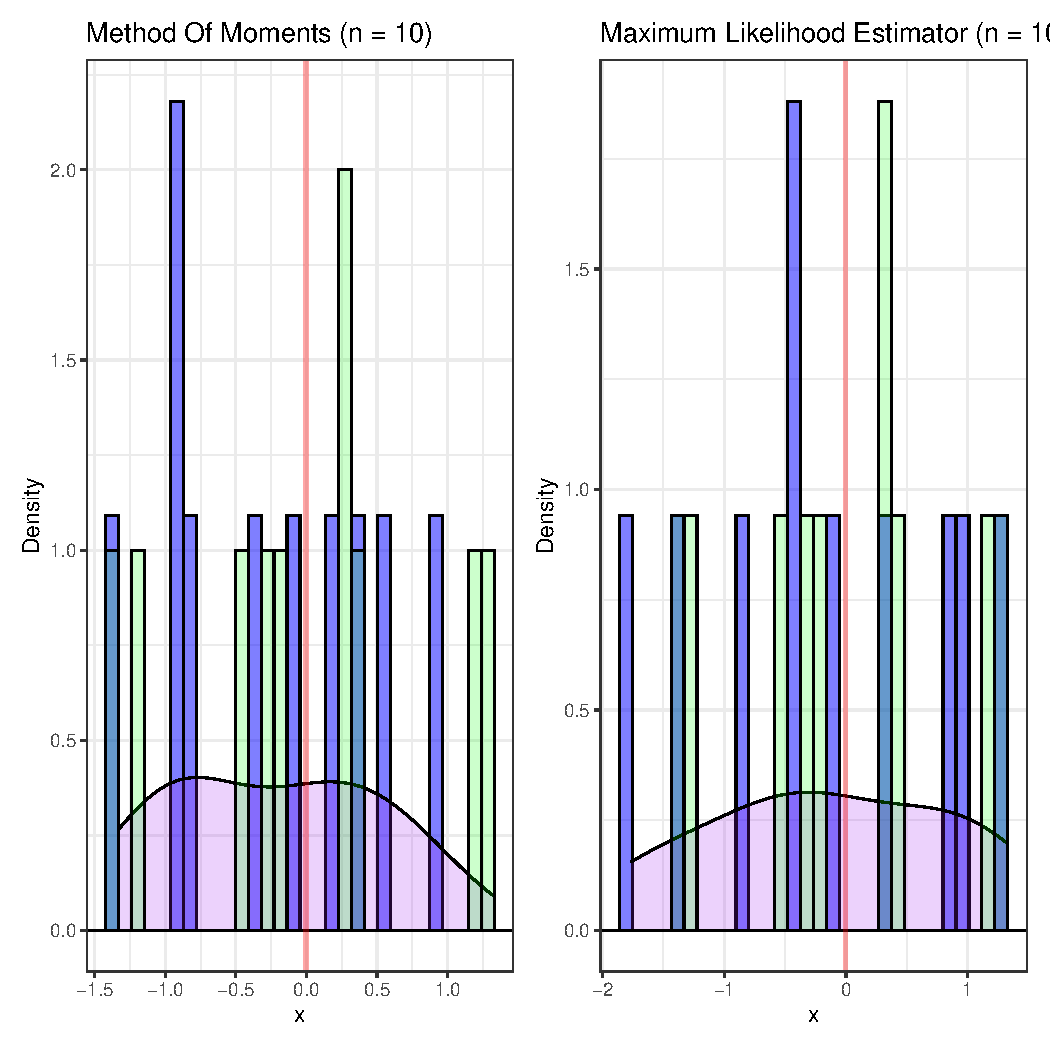
\includegraphics[width=\maxwidth]{figure/unnamed-chunk-24-1} 
\begin{kframe}\begin{alltt}
\hlstd{dat1_h} \hlkwb{<-} \hlkwd{ggplot}\hlstd{(}\hlkwc{data}\hlstd{=dat1,} \hlkwd{aes}\hlstd{(}\hlkwc{x}\hlstd{=x))}\hlopt{+}
  \hlkwd{geom_histogram}\hlstd{(}\hlkwc{color}\hlstd{=}\hlstr{"black"}\hlstd{,} \hlkwc{fill} \hlstd{=} \hlstr{"lightblue"}\hlstd{,} \hlkwc{alpha} \hlstd{=} \hlnum{0.5}\hlstd{,} \hlkwc{binwidth} \hlstd{=} \hlnum{0.2}\hlstd{,} \hlkwd{aes}\hlstd{(}\hlkwc{y}\hlstd{=..density..))}\hlopt{+}
  \hlkwd{geom_hline}\hlstd{(}\hlkwc{yintercept}\hlstd{=}\hlnum{0}\hlstd{)}\hlopt{+}
  \hlkwd{geom_density}\hlstd{(}\hlkwc{alpha}\hlstd{=}\hlnum{.2}\hlstd{,} \hlkwc{fill}\hlstd{=}\hlstr{"purple"}\hlstd{)} \hlopt{+}
  \hlkwd{theme_bw}\hlstd{()}\hlopt{+} \hlkwd{xlab}\hlstd{(}\hlstr{"x"}\hlstd{)}\hlopt{+} \hlkwd{ylab}\hlstd{(}\hlstr{"Density"}\hlstd{)}\hlopt{+}
  \hlkwd{ggtitle}\hlstd{(}\hlstr{"Normal Distrubution (n = 10)"}\hlstd{)} \hlopt{+}
  \hlkwd{geom_vline}\hlstd{(}\hlkwc{xintercept} \hlstd{=} \hlkwd{mean}\hlstd{(dat1}\hlopt{$}\hlstd{x),} \hlkwc{alpha}\hlstd{=}\hlnum{0.35}\hlstd{,} \hlkwc{color}\hlstd{=}\hlstr{"red"}\hlstd{,}\hlkwc{size}\hlstd{=}\hlnum{1}\hlstd{)}

\hlstd{dat1}\hlkwb{<-}\hlstd{dat1} \hlopt \hlkwd{mutate}\hlstd{(}\hlkwc{n} \hlstd{=} \hlkwd{seq}\hlstd{(}\hlnum{1}\hlstd{,obs[}\hlnum{1}\hlstd{],}\hlnum{1}\hlstd{))}

\hlstd{dat1_p} \hlkwb{<-} \hlkwd{ggplot}\hlstd{(}\hlkwc{data}\hlstd{=dat1,} \hlkwd{aes}\hlstd{(}\hlkwc{x}\hlstd{=n,} \hlkwc{y}\hlstd{=x))}\hlopt{+}
  \hlkwd{geom_line}\hlstd{()}\hlopt{+}
  \hlkwd{geom_hline}\hlstd{(}\hlkwc{yintercept}\hlstd{=}\hlnum{0}\hlstd{)}\hlopt{+}
  \hlkwd{geom_hline}\hlstd{(}\hlkwc{yintercept} \hlstd{=} \hlkwd{mean}\hlstd{(dat1}\hlopt{$}\hlstd{x),} \hlkwc{alpha}\hlstd{=}\hlnum{0.35}\hlstd{,} \hlkwc{color}\hlstd{=}\hlstr{"red"}\hlstd{,}\hlkwc{size}\hlstd{=}\hlnum{1}\hlstd{)} \hlopt{+}
  \hlkwd{theme_bw}\hlstd{()}\hlopt{+} \hlkwd{xlab}\hlstd{(}\hlstr{"n"}\hlstd{)}\hlopt{+} \hlkwd{ylab}\hlstd{(}\hlstr{"x"}\hlstd{)}\hlopt{+} \hlkwd{ggtitle}\hlstd{(}\hlstr{"Normal Distrubution (n = 10)"}\hlstd{)}

\hlstd{dat1_h} \hlopt{+} \hlstd{dat1_p}
\end{alltt}
\end{kframe}
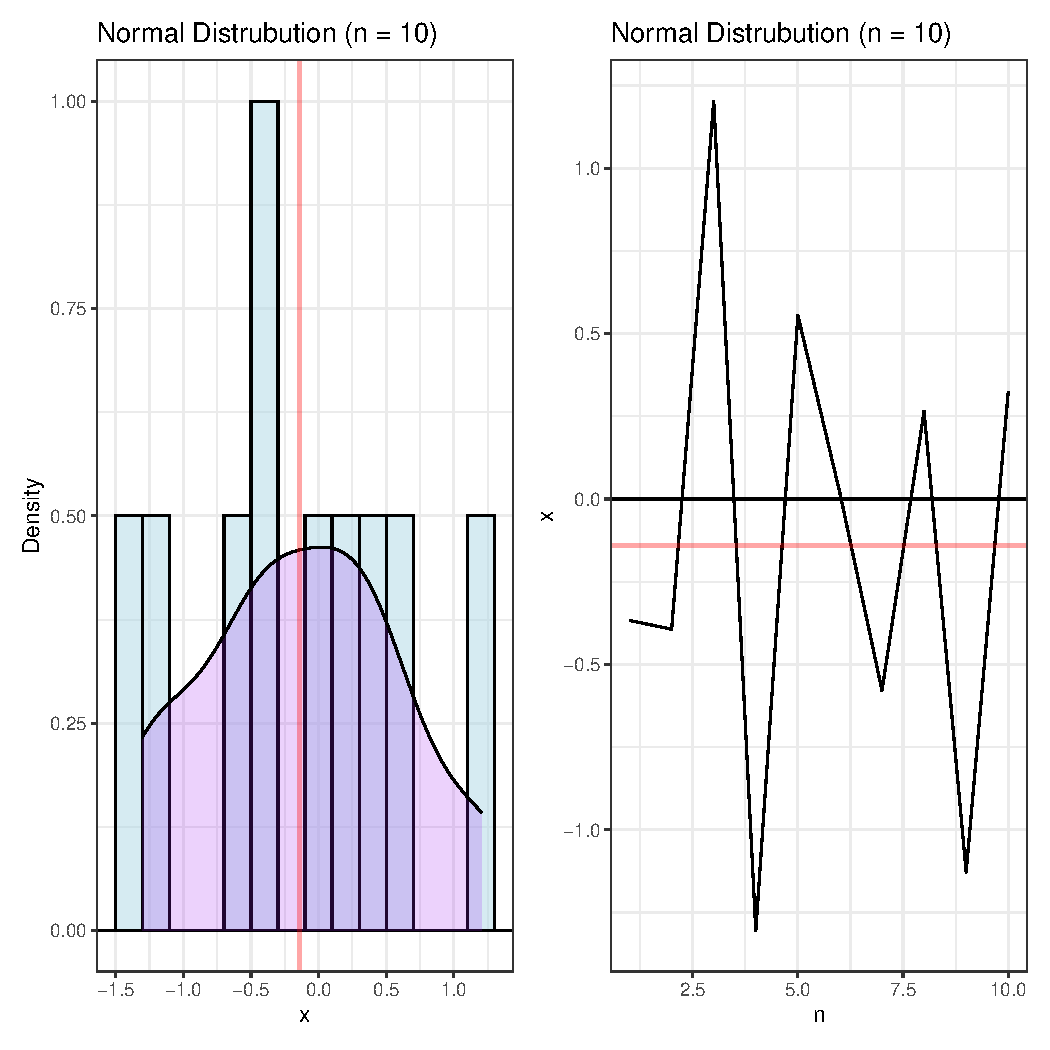
\includegraphics[width=\maxwidth]{figure/unnamed-chunk-24-2} 
\end{knitrout}
  %%%%%%%%%%%%%%%%%%%%%%%%%%%%%%%%%%%%%%%%%%%%%%%%%%%%%%%%%%%%%%%%%%%%%%%%%%%%%%%%%%%%%%%%%%%
  %%%%%%%%%  Part (d)
  %%%%%%%%%%%%%%%%%%%%%%%%%%%%%%%%%%%%%%%%%%%%%%%%%%%%%%%%%%%%%%%%%%%%%%%%%%%%%%%%%%%%%%%%%%%
  \item Generate a random sample of size $n=25$ for your two sets of parameter(s).
\begin{knitrout}
\definecolor{shadecolor}{rgb}{0.969, 0.969, 0.969}\color{fgcolor}\begin{kframe}
\begin{alltt}
\hlstd{dat2} \hlkwb{<-} \hlkwd{data.frame}\hlstd{(}\hlkwc{x} \hlstd{=} \hlkwd{rnorm}\hlstd{(}\hlkwc{n} \hlstd{= obs[}\hlnum{2}\hlstd{],} \hlkwc{mean} \hlstd{=} \hlnum{0}\hlstd{,} \hlkwc{sd} \hlstd{=} \hlnum{1}\hlstd{))}
\end{alltt}
\end{kframe}
\end{knitrout}
  Calculate the method of moments estimator(s) and maximum likelihood estimator(s). 
\begin{knitrout}
\definecolor{shadecolor}{rgb}{0.969, 0.969, 0.969}\color{fgcolor}\begin{kframe}
\begin{alltt}
\hlstd{mom2} \hlkwb{<-} \hlkwd{nleqslv}\hlstd{(}\hlkwc{x} \hlstd{=} \hlkwd{c}\hlstd{(}\hlnum{0}\hlstd{,}\hlnum{1}\hlstd{),}\hlkwc{fn} \hlstd{= norm.mom,} \hlkwc{data} \hlstd{= dat2}\hlopt{$}\hlstd{x)}
\hlstd{mle2} \hlkwb{<-} \hlkwd{optim}\hlstd{(}\hlkwc{par} \hlstd{=} \hlkwd{c}\hlstd{(}\hlnum{0}\hlstd{,}\hlnum{1}\hlstd{),} \hlkwc{fn} \hlstd{= norm.ll,} \hlkwc{data}\hlstd{=dat2}\hlopt{$}\hlstd{x)}
\end{alltt}
\end{kframe}
\end{knitrout}
  In a $1 \times 2$ grid, plot a histogram of each set of data with (1) the method 
  of moments estimated distribution, (2) the maximum likelihood estimated distribution, 
  and superimpose the true distribution in both.
\begin{knitrout}
\definecolor{shadecolor}{rgb}{0.969, 0.969, 0.969}\color{fgcolor}\begin{kframe}
\begin{alltt}
\hlstd{mom_dat2} \hlkwb{<-} \hlkwd{data.frame}\hlstd{(}\hlkwc{x} \hlstd{=} \hlkwd{rnorm}\hlstd{(}\hlkwc{n} \hlstd{= obs[}\hlnum{2}\hlstd{],} \hlkwc{mean} \hlstd{= mom2}\hlopt{$}\hlstd{x[}\hlnum{1}\hlstd{],} \hlkwc{sd} \hlstd{= mom2}\hlopt{$}\hlstd{x[}\hlnum{2}\hlstd{]))}
\hlstd{mom2_p} \hlkwb{<-} \hlkwd{ggplot}\hlstd{(}\hlkwc{data}\hlstd{=mom_dat2,} \hlkwd{aes}\hlstd{(}\hlkwc{x}\hlstd{=x))}\hlopt{+} \hlkwd{geom_histogram}\hlstd{(}\hlkwc{color}\hlstd{=}\hlstr{"black"}\hlstd{,} \hlkwc{fill} \hlstd{=} \hlstr{"blue"}\hlstd{,} \hlkwc{alpha} \hlstd{=} \hlnum{0.5}\hlstd{,} \hlkwd{aes}\hlstd{(}\hlkwc{y}\hlstd{=..density..))}\hlopt{+} \hlkwd{geom_hline}\hlstd{(}\hlkwc{yintercept}\hlstd{=}\hlnum{0}\hlstd{)}\hlopt{+} \hlkwd{geom_density}\hlstd{(}\hlkwc{alpha}\hlstd{=}\hlnum{.2}\hlstd{,} \hlkwc{fill}\hlstd{=}\hlstr{"purple"}\hlstd{)} \hlopt{+} \hlkwd{theme_bw}\hlstd{()}\hlopt{+} \hlkwd{xlab}\hlstd{(}\hlstr{"x"}\hlstd{)}\hlopt{+} \hlkwd{ylab}\hlstd{(}\hlstr{"Density"}\hlstd{)}\hlopt{+} \hlkwd{ggtitle}\hlstd{(}\hlstr{"Method Of Moments (n = 25)"}\hlstd{)} \hlopt{+} \hlkwd{geom_histogram}\hlstd{(}\hlkwd{aes}\hlstd{(}\hlkwc{x} \hlstd{= dat2}\hlopt{$}\hlstd{x,} \hlkwc{y}\hlstd{=..density..),} \hlkwc{color}\hlstd{=}\hlstr{"black"}\hlstd{,} \hlkwc{fill} \hlstd{=} \hlstr{"green"}\hlstd{,} \hlkwc{alpha} \hlstd{=} \hlnum{0.2}\hlstd{)} \hlopt{+} \hlkwd{geom_vline}\hlstd{(}\hlkwc{xintercept} \hlstd{=} \hlkwd{mean}\hlstd{(dat2}\hlopt{$}\hlstd{x),} \hlkwc{alpha}\hlstd{=}\hlnum{0.35}\hlstd{,} \hlkwc{color}\hlstd{=}\hlstr{"red"}\hlstd{,}\hlkwc{size}\hlstd{=}\hlnum{1}\hlstd{)}

\hlstd{mle_dat2} \hlkwb{<-} \hlkwd{data.frame}\hlstd{(}\hlkwc{x} \hlstd{=} \hlkwd{rnorm}\hlstd{(}\hlkwc{n} \hlstd{= obs[}\hlnum{2}\hlstd{],} \hlkwc{mean} \hlstd{= mle2}\hlopt{$}\hlstd{par[}\hlnum{1}\hlstd{],} \hlkwc{sd} \hlstd{= mle2}\hlopt{$}\hlstd{par[}\hlnum{2}\hlstd{]))}
\hlstd{mle2_p} \hlkwb{<-} \hlkwd{ggplot}\hlstd{(}\hlkwc{data}\hlstd{=mle_dat2,} \hlkwd{aes}\hlstd{(}\hlkwc{x}\hlstd{=x))}\hlopt{+} \hlkwd{geom_histogram}\hlstd{(}\hlkwc{color}\hlstd{=}\hlstr{"black"}\hlstd{,} \hlkwc{fill} \hlstd{=} \hlstr{"blue"}\hlstd{,} \hlkwc{alpha} \hlstd{=} \hlnum{0.5}\hlstd{,} \hlkwd{aes}\hlstd{(}\hlkwc{y}\hlstd{=..density..))}\hlopt{+} \hlkwd{geom_hline}\hlstd{(}\hlkwc{yintercept}\hlstd{=}\hlnum{0}\hlstd{)}\hlopt{+} \hlkwd{geom_density}\hlstd{(}\hlkwc{alpha}\hlstd{=}\hlnum{.2}\hlstd{,} \hlkwc{fill}\hlstd{=}\hlstr{"purple"}\hlstd{)} \hlopt{+} \hlkwd{theme_bw}\hlstd{()}\hlopt{+} \hlkwd{xlab}\hlstd{(}\hlstr{"x"}\hlstd{)}\hlopt{+} \hlkwd{ylab}\hlstd{(}\hlstr{"Density"}\hlstd{)}\hlopt{+} \hlkwd{ggtitle}\hlstd{(}\hlstr{"Maximum Likelihood Estimator (n = 25)"}\hlstd{)} \hlopt{+} \hlkwd{geom_histogram}\hlstd{(}\hlkwd{aes}\hlstd{(}\hlkwc{x} \hlstd{= dat2}\hlopt{$}\hlstd{x,} \hlkwc{y}\hlstd{=..density..),} \hlkwc{color}\hlstd{=}\hlstr{"black"}\hlstd{,} \hlkwc{fill} \hlstd{=} \hlstr{"green"}\hlstd{,} \hlkwc{alpha} \hlstd{=} \hlnum{0.2}\hlstd{)} \hlopt{+} \hlkwd{geom_vline}\hlstd{(}\hlkwc{xintercept} \hlstd{=} \hlkwd{mean}\hlstd{(dat2}\hlopt{$}\hlstd{x),} \hlkwc{alpha}\hlstd{=}\hlnum{0.35}\hlstd{,} \hlkwc{color}\hlstd{=}\hlstr{"red"}\hlstd{,}\hlkwc{size}\hlstd{=}\hlnum{1}\hlstd{)}

\hlstd{mom2_p} \hlopt{+} \hlstd{mle2_p}
\end{alltt}


{\ttfamily\noindent\itshape\color{messagecolor}{\#\# `stat\_bin()` using `bins = 30`. Pick better value with `binwidth`.\\\#\# `stat\_bin()` using `bins = 30`. Pick better value with `binwidth`.\\\#\# `stat\_bin()` using `bins = 30`. Pick better value with `binwidth`.\\\#\# `stat\_bin()` using `bins = 30`. Pick better value with `binwidth`.}}\end{kframe}
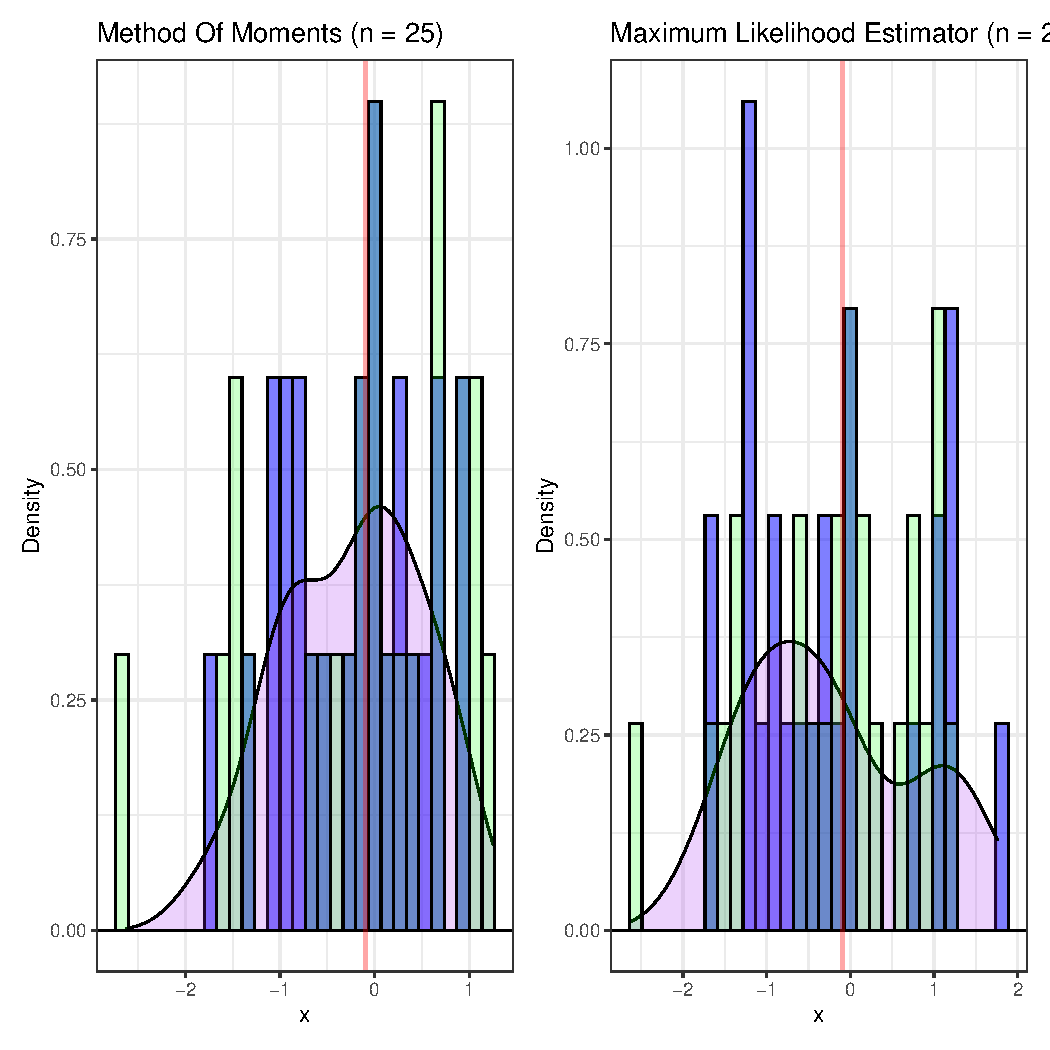
\includegraphics[width=\maxwidth]{figure/unnamed-chunk-27-1} 
\begin{kframe}\begin{alltt}
\hlstd{dat2_h} \hlkwb{<-} \hlkwd{ggplot}\hlstd{(}\hlkwc{data}\hlstd{=dat2,} \hlkwd{aes}\hlstd{(}\hlkwc{x}\hlstd{=x))}\hlopt{+} \hlkwd{geom_histogram}\hlstd{(}\hlkwc{color}\hlstd{=}\hlstr{"black"}\hlstd{,} \hlkwc{fill} \hlstd{=} \hlstr{"lightblue"}\hlstd{,} \hlkwc{alpha} \hlstd{=} \hlnum{0.5}\hlstd{,} \hlkwc{binwidth} \hlstd{=} \hlnum{0.2}\hlstd{,} \hlkwd{aes}\hlstd{(}\hlkwc{y}\hlstd{=..density..))}\hlopt{+} \hlkwd{geom_hline}\hlstd{(}\hlkwc{yintercept}\hlstd{=}\hlnum{0}\hlstd{)}\hlopt{+} \hlkwd{geom_density}\hlstd{(}\hlkwc{alpha}\hlstd{=}\hlnum{.2}\hlstd{,} \hlkwc{fill}\hlstd{=}\hlstr{"purple"}\hlstd{)} \hlopt{+} \hlkwd{theme_bw}\hlstd{()}\hlopt{+} \hlkwd{xlab}\hlstd{(}\hlstr{"x"}\hlstd{)}\hlopt{+} \hlkwd{ylab}\hlstd{(}\hlstr{"Density"}\hlstd{)}\hlopt{+} \hlkwd{ggtitle}\hlstd{(}\hlstr{"Normal Distrubution (n = 25)"}\hlstd{)} \hlopt{+} \hlkwd{geom_vline}\hlstd{(}\hlkwc{xintercept} \hlstd{=} \hlkwd{mean}\hlstd{(dat2}\hlopt{$}\hlstd{x),} \hlkwc{alpha}\hlstd{=}\hlnum{0.35}\hlstd{,} \hlkwc{color}\hlstd{=}\hlstr{"red"}\hlstd{,}\hlkwc{size}\hlstd{=}\hlnum{1}\hlstd{)}

\hlstd{dat2} \hlkwb{<-}\hlstd{dat2} \hlopt \hlkwd{mutate}\hlstd{(}\hlkwc{n} \hlstd{=} \hlkwd{seq}\hlstd{(}\hlnum{1}\hlstd{,obs[}\hlnum{2}\hlstd{],}\hlnum{1}\hlstd{))}
\hlstd{dat2_p} \hlkwb{<-} \hlkwd{ggplot}\hlstd{(}\hlkwc{data}\hlstd{=dat2,} \hlkwd{aes}\hlstd{(}\hlkwc{x}\hlstd{=n,} \hlkwc{y}\hlstd{=x))}\hlopt{+} \hlkwd{geom_line}\hlstd{()}\hlopt{+} \hlkwd{geom_hline}\hlstd{(}\hlkwc{yintercept}\hlstd{=}\hlnum{0}\hlstd{)}\hlopt{+} \hlkwd{geom_hline}\hlstd{(}\hlkwc{yintercept} \hlstd{=} \hlkwd{mean}\hlstd{(dat2}\hlopt{$}\hlstd{x),} \hlkwc{alpha}\hlstd{=}\hlnum{0.35}\hlstd{,} \hlkwc{color}\hlstd{=}\hlstr{"red"}\hlstd{,}\hlkwc{size}\hlstd{=}\hlnum{1}\hlstd{)} \hlopt{+} \hlkwd{theme_bw}\hlstd{()}\hlopt{+} \hlkwd{xlab}\hlstd{(}\hlstr{"n"}\hlstd{)}\hlopt{+} \hlkwd{ylab}\hlstd{(}\hlstr{"x"}\hlstd{)}\hlopt{+} \hlkwd{ggtitle}\hlstd{(}\hlstr{"Normal Distrubution (n = 25)"}\hlstd{)}

\hlstd{dat2_h} \hlopt{+} \hlstd{dat2_p}
\end{alltt}
\end{kframe}
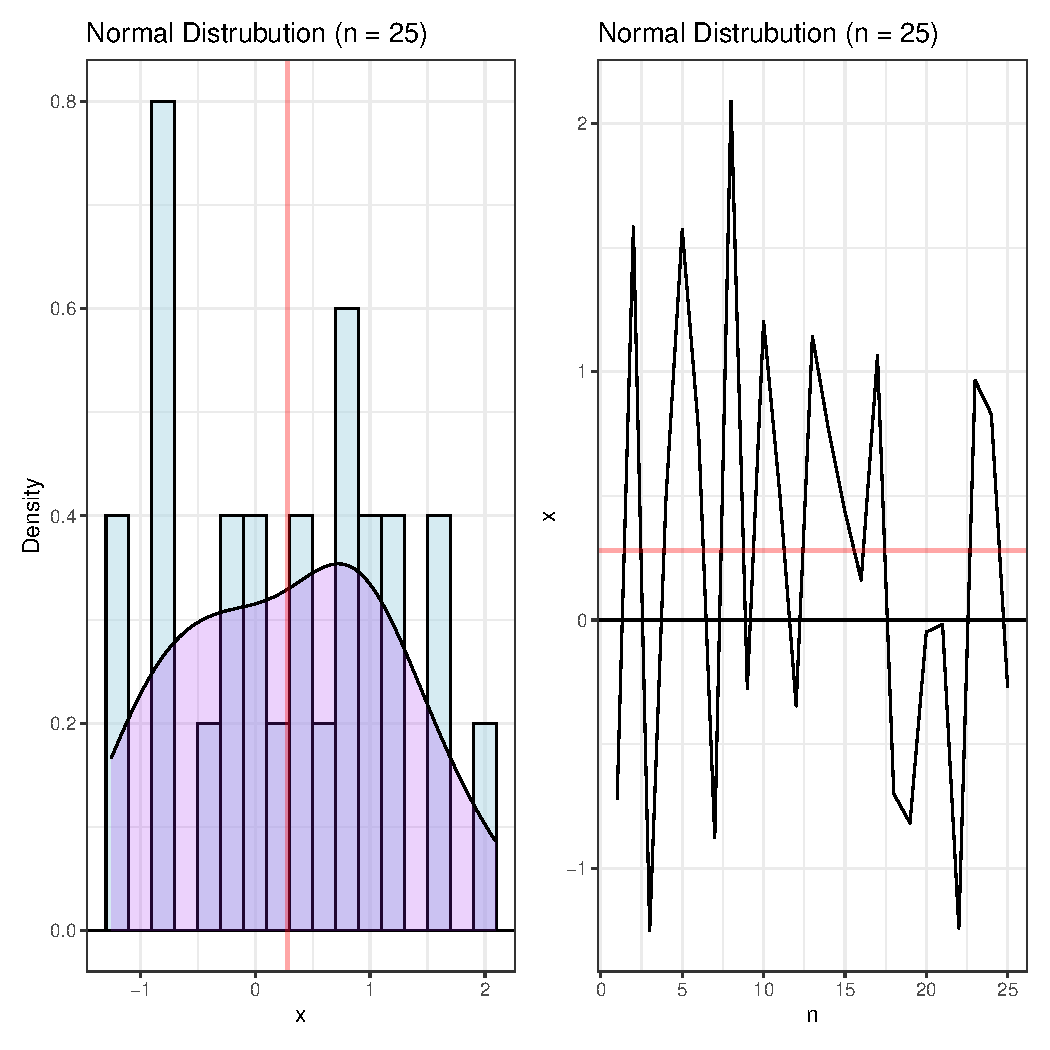
\includegraphics[width=\maxwidth]{figure/unnamed-chunk-27-2} 
\end{knitrout}
  %%%%%%%%%%%%%%%%%%%%%%%%%%%%%%%%%%%%%%%%%%%%%%%%%%%%%%%%%%%%%%%%%%%%%%%%%%%%%%%%%%%%%%%%%%%
  %%%%%%%%%  Part (e)
  %%%%%%%%%%%%%%%%%%%%%%%%%%%%%%%%%%%%%%%%%%%%%%%%%%%%%%%%%%%%%%%%%%%%%%%%%%%%%%%%%%%%%%%%%%%
  \item Generate a random sample of size $n=100$ for your two sets of parameter(s). 
\begin{knitrout}
\definecolor{shadecolor}{rgb}{0.969, 0.969, 0.969}\color{fgcolor}\begin{kframe}
\begin{alltt}
\hlstd{dat3} \hlkwb{<-} \hlkwd{data.frame}\hlstd{(}\hlkwc{x} \hlstd{=} \hlkwd{rnorm}\hlstd{(}\hlkwc{n} \hlstd{= obs[}\hlnum{3}\hlstd{],} \hlkwc{mean} \hlstd{=} \hlnum{0}\hlstd{,} \hlkwc{sd} \hlstd{=} \hlnum{1}\hlstd{))}
\end{alltt}
\end{kframe}
\end{knitrout}
  Calculate the method of moments estimator(s) and maximum likelihood estimator(s).
\begin{knitrout}
\definecolor{shadecolor}{rgb}{0.969, 0.969, 0.969}\color{fgcolor}\begin{kframe}
\begin{alltt}
\hlstd{mom3} \hlkwb{<-} \hlkwd{nleqslv}\hlstd{(}\hlkwc{x} \hlstd{=} \hlkwd{c}\hlstd{(}\hlnum{0}\hlstd{,}\hlnum{1}\hlstd{),}\hlkwc{fn} \hlstd{= norm.mom,} \hlkwc{data} \hlstd{= dat3}\hlopt{$}\hlstd{x)}
\hlstd{mle3} \hlkwb{<-} \hlkwd{optim}\hlstd{(}\hlkwc{par} \hlstd{=} \hlkwd{c}\hlstd{(}\hlnum{0}\hlstd{,}\hlnum{1}\hlstd{),} \hlkwc{fn} \hlstd{= norm.ll,} \hlkwc{data}\hlstd{=dat3}\hlopt{$}\hlstd{x)}
\end{alltt}
\end{kframe}
\end{knitrout}
  In a $1 \times 2$ grid, plot a histogram of each set of data with (1) the method 
  of moments estimated distribution, (2) the maximum likelihood estimated distribution,
  and superimpose the true distribution in both.
\begin{knitrout}
\definecolor{shadecolor}{rgb}{0.969, 0.969, 0.969}\color{fgcolor}\begin{kframe}
\begin{alltt}
\hlstd{mom_dat3} \hlkwb{<-} \hlkwd{data.frame}\hlstd{(}\hlkwc{x} \hlstd{=} \hlkwd{rnorm}\hlstd{(}\hlkwc{n} \hlstd{= obs[}\hlnum{3}\hlstd{],} \hlkwc{mean} \hlstd{= mom3}\hlopt{$}\hlstd{x[}\hlnum{1}\hlstd{],} \hlkwc{sd} \hlstd{= mom3}\hlopt{$}\hlstd{x[}\hlnum{2}\hlstd{]))}
\hlstd{mom3_p} \hlkwb{<-} \hlkwd{ggplot}\hlstd{(}\hlkwc{data}\hlstd{=mom_dat3,} \hlkwd{aes}\hlstd{(}\hlkwc{x}\hlstd{=x))}\hlopt{+} \hlkwd{geom_histogram}\hlstd{(}\hlkwc{color}\hlstd{=}\hlstr{"black"}\hlstd{,} \hlkwc{fill} \hlstd{=} \hlstr{"blue"}\hlstd{,} \hlkwc{alpha} \hlstd{=} \hlnum{0.5}\hlstd{,} \hlkwd{aes}\hlstd{(}\hlkwc{y}\hlstd{=..density..))}\hlopt{+} \hlkwd{geom_hline}\hlstd{(}\hlkwc{yintercept}\hlstd{=}\hlnum{0}\hlstd{)}\hlopt{+} \hlkwd{geom_density}\hlstd{(}\hlkwc{alpha}\hlstd{=}\hlnum{.2}\hlstd{,} \hlkwc{fill}\hlstd{=}\hlstr{"purple"}\hlstd{)} \hlopt{+} \hlkwd{theme_bw}\hlstd{()}\hlopt{+} \hlkwd{xlab}\hlstd{(}\hlstr{"x"}\hlstd{)}\hlopt{+} \hlkwd{ylab}\hlstd{(}\hlstr{"Density"}\hlstd{)}\hlopt{+} \hlkwd{ggtitle}\hlstd{(}\hlstr{"Method of Moments (n = 100)"}\hlstd{)} \hlopt{+} \hlkwd{geom_histogram}\hlstd{(}\hlkwd{aes}\hlstd{(}\hlkwc{x} \hlstd{= dat3}\hlopt{$}\hlstd{x,} \hlkwc{y}\hlstd{=..density..),} \hlkwc{color}\hlstd{=}\hlstr{"black"}\hlstd{,} \hlkwc{fill} \hlstd{=} \hlstr{"green"}\hlstd{,} \hlkwc{alpha} \hlstd{=} \hlnum{0.2}\hlstd{)} \hlopt{+} \hlkwd{geom_vline}\hlstd{(}\hlkwc{xintercept} \hlstd{=} \hlkwd{mean}\hlstd{(dat3}\hlopt{$}\hlstd{x),} \hlkwc{alpha}\hlstd{=}\hlnum{0.35}\hlstd{,} \hlkwc{color}\hlstd{=}\hlstr{"red"}\hlstd{,}\hlkwc{size}\hlstd{=}\hlnum{1}\hlstd{)}

\hlstd{mle_dat3} \hlkwb{<-} \hlkwd{data.frame}\hlstd{(}\hlkwc{x} \hlstd{=} \hlkwd{rnorm}\hlstd{(}\hlkwc{n} \hlstd{= obs[}\hlnum{3}\hlstd{],} \hlkwc{mean} \hlstd{= mle3}\hlopt{$}\hlstd{par[}\hlnum{1}\hlstd{],} \hlkwc{sd} \hlstd{= mle3}\hlopt{$}\hlstd{par[}\hlnum{2}\hlstd{]))}
\hlstd{mle3_p} \hlkwb{<-} \hlkwd{ggplot}\hlstd{(}\hlkwc{data}\hlstd{=mle_dat3,} \hlkwd{aes}\hlstd{(}\hlkwc{x}\hlstd{=x))}\hlopt{+} \hlkwd{geom_histogram}\hlstd{(}\hlkwc{color}\hlstd{=}\hlstr{"black"}\hlstd{,} \hlkwc{fill} \hlstd{=} \hlstr{"blue"}\hlstd{,} \hlkwc{alpha} \hlstd{=} \hlnum{0.5}\hlstd{,} \hlkwd{aes}\hlstd{(}\hlkwc{y}\hlstd{=..density..))}\hlopt{+} \hlkwd{geom_hline}\hlstd{(}\hlkwc{yintercept}\hlstd{=}\hlnum{0}\hlstd{)}\hlopt{+} \hlkwd{geom_density}\hlstd{(}\hlkwc{alpha}\hlstd{=}\hlnum{.2}\hlstd{,} \hlkwc{fill}\hlstd{=}\hlstr{"purple"}\hlstd{)} \hlopt{+} \hlkwd{theme_bw}\hlstd{()}\hlopt{+} \hlkwd{xlab}\hlstd{(}\hlstr{"x"}\hlstd{)}\hlopt{+} \hlkwd{ylab}\hlstd{(}\hlstr{"Density"}\hlstd{)}\hlopt{+} \hlkwd{ggtitle}\hlstd{(}\hlstr{"Maximum Likelihood Estimator (n = 100)"}\hlstd{)} \hlopt{+} \hlkwd{geom_histogram}\hlstd{(}\hlkwd{aes}\hlstd{(}\hlkwc{x} \hlstd{= dat3}\hlopt{$}\hlstd{x,} \hlkwc{y}\hlstd{=..density..),} \hlkwc{color}\hlstd{=}\hlstr{"black"}\hlstd{,} \hlkwc{fill} \hlstd{=} \hlstr{"green"}\hlstd{,} \hlkwc{alpha} \hlstd{=} \hlnum{0.2}\hlstd{)} \hlopt{+} \hlkwd{geom_vline}\hlstd{(}\hlkwc{xintercept} \hlstd{=} \hlkwd{mean}\hlstd{(dat3}\hlopt{$}\hlstd{x),} \hlkwc{alpha}\hlstd{=}\hlnum{0.35}\hlstd{,} \hlkwc{color}\hlstd{=}\hlstr{"red"}\hlstd{,}\hlkwc{size}\hlstd{=}\hlnum{1}\hlstd{)}

\hlstd{mom3_p} \hlopt{+} \hlstd{mle3_p}
\end{alltt}


{\ttfamily\noindent\itshape\color{messagecolor}{\#\# `stat\_bin()` using `bins = 30`. Pick better value with `binwidth`.\\\#\# `stat\_bin()` using `bins = 30`. Pick better value with `binwidth`.\\\#\# `stat\_bin()` using `bins = 30`. Pick better value with `binwidth`.\\\#\# `stat\_bin()` using `bins = 30`. Pick better value with `binwidth`.}}\end{kframe}
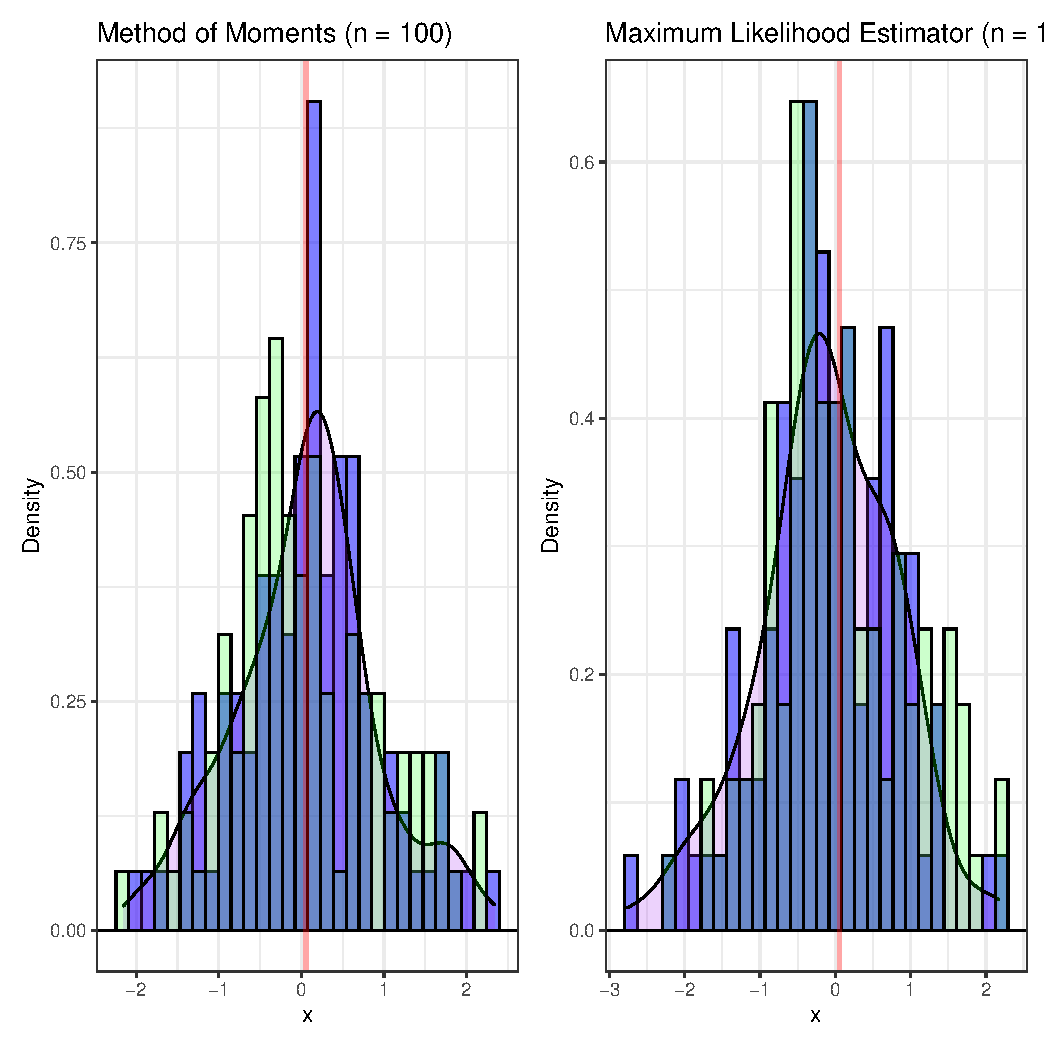
\includegraphics[width=\maxwidth]{figure/unnamed-chunk-30-1} 
\begin{kframe}\begin{alltt}
\hlstd{dat3_h} \hlkwb{<-} \hlkwd{ggplot}\hlstd{(}\hlkwc{data}\hlstd{=dat3,} \hlkwd{aes}\hlstd{(}\hlkwc{x}\hlstd{=x))}\hlopt{+} \hlkwd{geom_histogram}\hlstd{(}\hlkwc{color}\hlstd{=}\hlstr{"black"}\hlstd{,} \hlkwc{fill} \hlstd{=} \hlstr{"lightblue"}\hlstd{,} \hlkwc{alpha} \hlstd{=} \hlnum{0.5}\hlstd{,} \hlkwc{binwidth} \hlstd{=} \hlnum{0.2}\hlstd{,} \hlkwd{aes}\hlstd{(}\hlkwc{y}\hlstd{=..density..))}\hlopt{+} \hlkwd{geom_hline}\hlstd{(}\hlkwc{yintercept}\hlstd{=}\hlnum{0}\hlstd{)}\hlopt{+} \hlkwd{geom_density}\hlstd{(}\hlkwc{alpha}\hlstd{=}\hlnum{.2}\hlstd{,} \hlkwc{fill}\hlstd{=}\hlstr{"purple"}\hlstd{)} \hlopt{+} \hlkwd{theme_bw}\hlstd{()}\hlopt{+} \hlkwd{xlab}\hlstd{(}\hlstr{"x"}\hlstd{)}\hlopt{+} \hlkwd{ylab}\hlstd{(}\hlstr{"Density"}\hlstd{)}\hlopt{+} \hlkwd{ggtitle}\hlstd{(}\hlstr{"Normal Distrubution (n = 100)"}\hlstd{)}

\hlstd{dat3} \hlkwb{<-}\hlstd{dat3} \hlopt \hlkwd{mutate}\hlstd{(}\hlkwc{n} \hlstd{=} \hlkwd{seq}\hlstd{(}\hlnum{1}\hlstd{,obs[}\hlnum{3}\hlstd{],}\hlnum{1}\hlstd{))}
\hlstd{dat3_p} \hlkwb{<-} \hlkwd{ggplot}\hlstd{(}\hlkwc{data}\hlstd{=dat3,} \hlkwd{aes}\hlstd{(}\hlkwc{x}\hlstd{=n,} \hlkwc{y}\hlstd{=x))}\hlopt{+} \hlkwd{geom_line}\hlstd{()}\hlopt{+} \hlkwd{geom_hline}\hlstd{(}\hlkwc{yintercept}\hlstd{=}\hlnum{0}\hlstd{)}\hlopt{+} \hlkwd{geom_hline}\hlstd{(}\hlkwc{yintercept} \hlstd{=} \hlkwd{mean}\hlstd{(dat3}\hlopt{$}\hlstd{x),} \hlkwc{alpha}\hlstd{=}\hlnum{0.35}\hlstd{,} \hlkwc{color}\hlstd{=}\hlstr{"red"}\hlstd{,}\hlkwc{size}\hlstd{=}\hlnum{1}\hlstd{)} \hlopt{+} \hlkwd{theme_bw}\hlstd{()}\hlopt{+} \hlkwd{xlab}\hlstd{(}\hlstr{"n"}\hlstd{)}\hlopt{+} \hlkwd{ylab}\hlstd{(}\hlstr{"x"}\hlstd{)}\hlopt{+} \hlkwd{ggtitle}\hlstd{(}\hlstr{"Normal Distrubution (n = 100)"}\hlstd{)}

\hlstd{dat3_h} \hlopt{+} \hlstd{dat3_p}
\end{alltt}
\end{kframe}
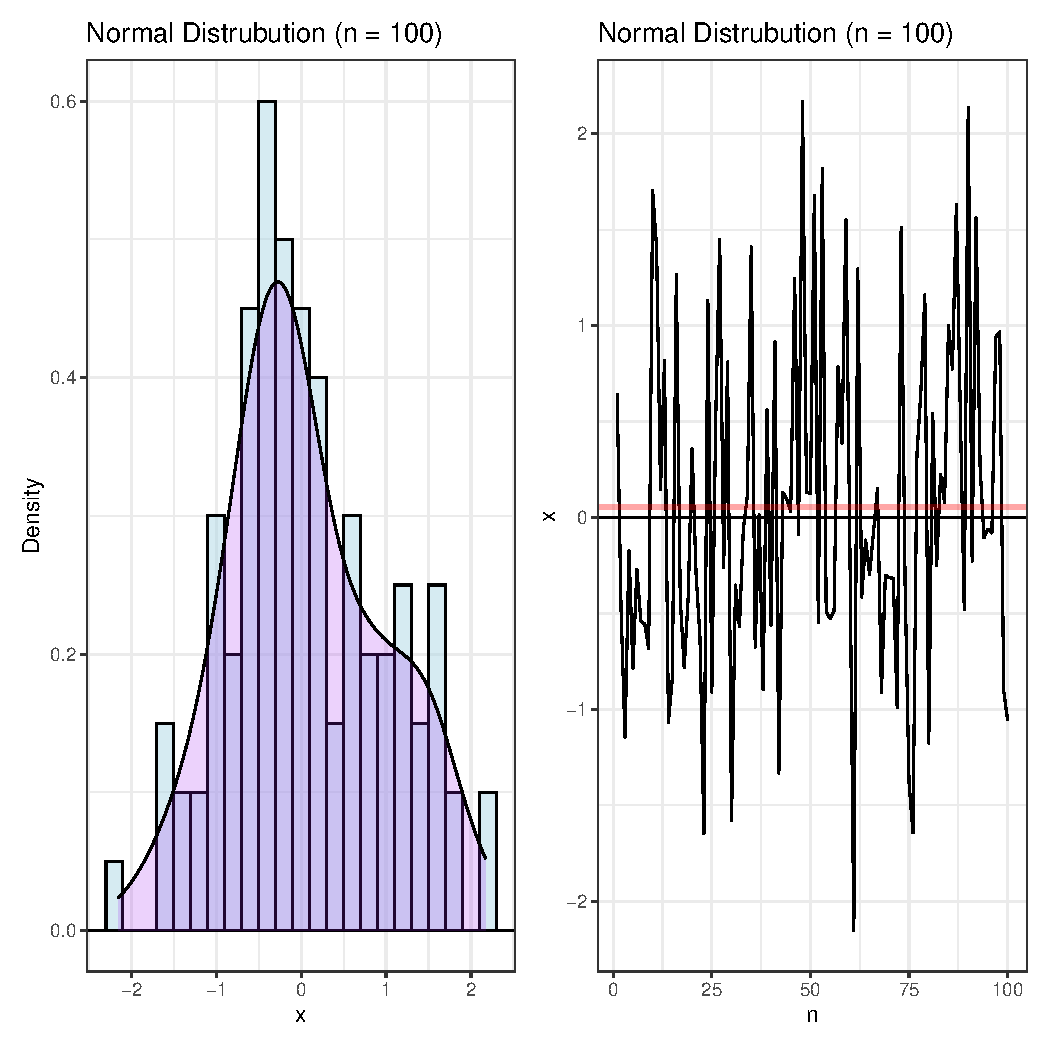
\includegraphics[width=\maxwidth]{figure/unnamed-chunk-30-2} 
\end{knitrout}
  %%%%%%%%%%%%%%%%%%%%%%%%%%%%%%%%%%%%%%%%%%%%%%%%%%%%%%%%%%%%%%%%%%%%%%%%%%%%%%%%%%%%%%%%%%%
  %%%%%%%%%  Part (f)
  %%%%%%%%%%%%%%%%%%%%%%%%%%%%%%%%%%%%%%%%%%%%%%%%%%%%%%%%%%%%%%%%%%%%%%%%%%%%%%%%%%%%%%%%%%%
  \item Generate a random sample of size $n=100$ for your two sets of parameter(s). 
\begin{knitrout}
\definecolor{shadecolor}{rgb}{0.969, 0.969, 0.969}\color{fgcolor}\begin{kframe}
\begin{alltt}
\hlstd{dat4} \hlkwb{<-} \hlkwd{data.frame}\hlstd{(}\hlkwc{x} \hlstd{=} \hlkwd{rnorm}\hlstd{(}\hlkwc{n} \hlstd{= obs[}\hlnum{4}\hlstd{],} \hlkwc{mean} \hlstd{=} \hlnum{0}\hlstd{,} \hlkwc{sd} \hlstd{=} \hlnum{1}\hlstd{))}
\end{alltt}
\end{kframe}
\end{knitrout}
  Calculate the method of moments estimator(s) and maximum likelihood estimator(s). 
\begin{knitrout}
\definecolor{shadecolor}{rgb}{0.969, 0.969, 0.969}\color{fgcolor}\begin{kframe}
\begin{alltt}
\hlstd{mom4} \hlkwb{<-} \hlkwd{nleqslv}\hlstd{(}\hlkwc{x} \hlstd{=} \hlkwd{c}\hlstd{(}\hlnum{0}\hlstd{,}\hlnum{1}\hlstd{),}\hlkwc{fn} \hlstd{= norm.mom,} \hlkwc{data} \hlstd{= dat4}\hlopt{$}\hlstd{x)}
\hlstd{mle4} \hlkwb{<-} \hlkwd{optim}\hlstd{(}\hlkwc{par} \hlstd{=} \hlkwd{c}\hlstd{(}\hlnum{0}\hlstd{,}\hlnum{1}\hlstd{),} \hlkwc{fn} \hlstd{= norm.ll,} \hlkwc{data}\hlstd{=dat4}\hlopt{$}\hlstd{x)}
\end{alltt}
\end{kframe}
\end{knitrout}
  In a $1 \times 2$ grid, plot a histogram of each set of data with (1) the method 
  of moments estimated distribution, (2) the maximum likelihood estimated distribution, 
  and superimpose the true distribution in both.
\begin{knitrout}
\definecolor{shadecolor}{rgb}{0.969, 0.969, 0.969}\color{fgcolor}\begin{kframe}
\begin{alltt}
\hlstd{mom_dat4} \hlkwb{<-} \hlkwd{data.frame}\hlstd{(}\hlkwc{x} \hlstd{=} \hlkwd{rnorm}\hlstd{(}\hlkwc{n} \hlstd{= obs[}\hlnum{4}\hlstd{],} \hlkwc{mean} \hlstd{= mom4}\hlopt{$}\hlstd{x[}\hlnum{1}\hlstd{],} \hlkwc{sd} \hlstd{= mom4}\hlopt{$}\hlstd{x[}\hlnum{2}\hlstd{]))}
\hlstd{mom4_p} \hlkwb{<-} \hlkwd{ggplot}\hlstd{(}\hlkwc{data}\hlstd{=mom_dat4,} \hlkwd{aes}\hlstd{(}\hlkwc{x}\hlstd{=x))}\hlopt{+} \hlkwd{geom_histogram}\hlstd{(}\hlkwc{color}\hlstd{=}\hlstr{"black"}\hlstd{,} \hlkwc{fill} \hlstd{=} \hlstr{"blue"}\hlstd{,} \hlkwc{alpha} \hlstd{=} \hlnum{0.5}\hlstd{,} \hlkwd{aes}\hlstd{(}\hlkwc{y}\hlstd{=..density..))}\hlopt{+} \hlkwd{geom_hline}\hlstd{(}\hlkwc{yintercept}\hlstd{=}\hlnum{0}\hlstd{)}\hlopt{+} \hlkwd{geom_density}\hlstd{(}\hlkwc{alpha}\hlstd{=}\hlnum{.2}\hlstd{,} \hlkwc{fill}\hlstd{=}\hlstr{"purple"}\hlstd{)} \hlopt{+} \hlkwd{theme_bw}\hlstd{()}\hlopt{+} \hlkwd{xlab}\hlstd{(}\hlstr{"x"}\hlstd{)}\hlopt{+} \hlkwd{ylab}\hlstd{(}\hlstr{"Density"}\hlstd{)}\hlopt{+} \hlkwd{ggtitle}\hlstd{(}\hlstr{"Method of Moments (n = 1000)"}\hlstd{)} \hlopt{+} \hlkwd{geom_histogram}\hlstd{(}\hlkwd{aes}\hlstd{(}\hlkwc{x} \hlstd{= dat4}\hlopt{$}\hlstd{x,} \hlkwc{y}\hlstd{=..density..),} \hlkwc{color}\hlstd{=}\hlstr{"black"}\hlstd{,} \hlkwc{fill} \hlstd{=} \hlstr{"green"}\hlstd{,} \hlkwc{alpha} \hlstd{=} \hlnum{0.2}\hlstd{)} \hlopt{+} \hlkwd{geom_vline}\hlstd{(}\hlkwc{xintercept} \hlstd{=} \hlkwd{mean}\hlstd{(dat4}\hlopt{$}\hlstd{x),} \hlkwc{alpha}\hlstd{=}\hlnum{0.35}\hlstd{,} \hlkwc{color}\hlstd{=}\hlstr{"red"}\hlstd{,}\hlkwc{size}\hlstd{=}\hlnum{1}\hlstd{)}

\hlstd{mle_dat4} \hlkwb{<-} \hlkwd{data.frame}\hlstd{(}\hlkwc{x} \hlstd{=} \hlkwd{rnorm}\hlstd{(}\hlkwc{n} \hlstd{= obs[}\hlnum{4}\hlstd{],} \hlkwc{mean} \hlstd{= mle4}\hlopt{$}\hlstd{par[}\hlnum{1}\hlstd{],} \hlkwc{sd} \hlstd{= mle4}\hlopt{$}\hlstd{par[}\hlnum{2}\hlstd{]))}
\hlstd{mle4_p} \hlkwb{<-} \hlkwd{ggplot}\hlstd{(}\hlkwc{data}\hlstd{=mle_dat4,} \hlkwd{aes}\hlstd{(}\hlkwc{x}\hlstd{=x))}\hlopt{+} \hlkwd{geom_histogram}\hlstd{(}\hlkwc{color}\hlstd{=}\hlstr{"black"}\hlstd{,} \hlkwc{fill} \hlstd{=} \hlstr{"blue"}\hlstd{,} \hlkwc{alpha} \hlstd{=} \hlnum{0.5}\hlstd{,} \hlkwd{aes}\hlstd{(}\hlkwc{y}\hlstd{=..density..))}\hlopt{+} \hlkwd{geom_hline}\hlstd{(}\hlkwc{yintercept}\hlstd{=}\hlnum{0}\hlstd{)}\hlopt{+} \hlkwd{geom_density}\hlstd{(}\hlkwc{alpha}\hlstd{=}\hlnum{.2}\hlstd{,} \hlkwc{fill}\hlstd{=}\hlstr{"purple"}\hlstd{)} \hlopt{+} \hlkwd{theme_bw}\hlstd{()}\hlopt{+} \hlkwd{xlab}\hlstd{(}\hlstr{"x"}\hlstd{)}\hlopt{+} \hlkwd{ylab}\hlstd{(}\hlstr{"Density"}\hlstd{)}\hlopt{+} \hlkwd{ggtitle}\hlstd{(}\hlstr{"Maximum Likelihood Estimator (n = 1000)"}\hlstd{)} \hlopt{+} \hlkwd{geom_vline}\hlstd{(}\hlkwc{xintercept} \hlstd{=} \hlkwd{mean}\hlstd{(dat4}\hlopt{$}\hlstd{x),} \hlkwc{alpha}\hlstd{=}\hlnum{0.35}\hlstd{,} \hlkwc{color}\hlstd{=}\hlstr{"red"}\hlstd{,}\hlkwc{size}\hlstd{=}\hlnum{1}\hlstd{)} \hlopt{+} \hlkwd{geom_histogram}\hlstd{(}\hlkwd{aes}\hlstd{(}\hlkwc{x} \hlstd{= dat4}\hlopt{$}\hlstd{x,} \hlkwc{y}\hlstd{=..density..),} \hlkwc{color}\hlstd{=}\hlstr{"black"}\hlstd{,} \hlkwc{fill} \hlstd{=} \hlstr{"green"}\hlstd{,} \hlkwc{alpha} \hlstd{=} \hlnum{0.2}\hlstd{)}

\hlstd{mom4_p} \hlopt{+} \hlstd{mle4_p}
\end{alltt}


{\ttfamily\noindent\itshape\color{messagecolor}{\#\# `stat\_bin()` using `bins = 30`. Pick better value with `binwidth`.\\\#\# `stat\_bin()` using `bins = 30`. Pick better value with `binwidth`.\\\#\# `stat\_bin()` using `bins = 30`. Pick better value with `binwidth`.\\\#\# `stat\_bin()` using `bins = 30`. Pick better value with `binwidth`.}}\end{kframe}
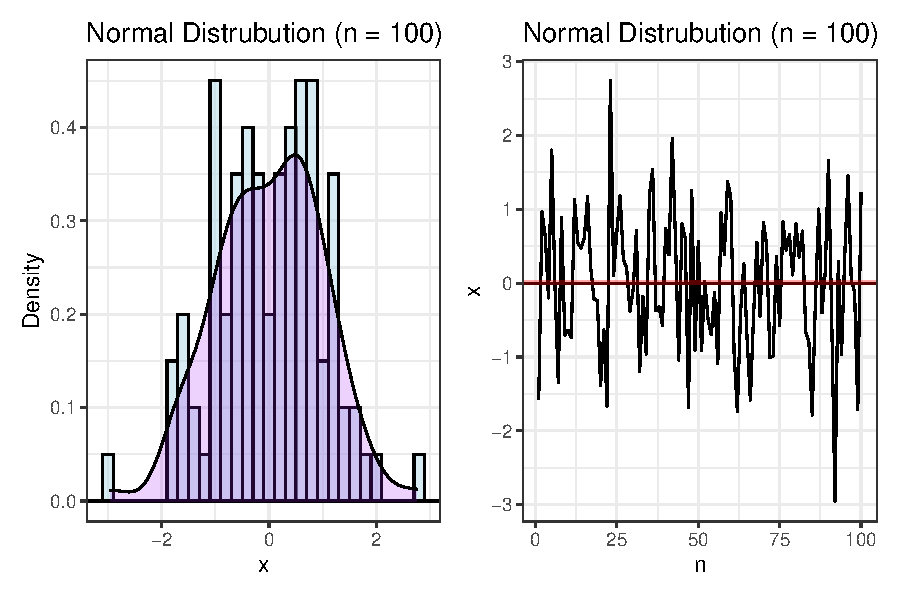
\includegraphics[width=\maxwidth]{figure/unnamed-chunk-33-1} 
\begin{kframe}\begin{alltt}
\hlstd{dat4_h} \hlkwb{<-} \hlkwd{ggplot}\hlstd{(}\hlkwc{data}\hlstd{=dat4,} \hlkwd{aes}\hlstd{(}\hlkwc{x}\hlstd{=x))}\hlopt{+} \hlkwd{geom_histogram}\hlstd{(}\hlkwc{color}\hlstd{=}\hlstr{"black"}\hlstd{,} \hlkwc{fill} \hlstd{=} \hlstr{"lightblue"}\hlstd{,} \hlkwc{alpha} \hlstd{=} \hlnum{0.5}\hlstd{,} \hlkwd{aes}\hlstd{(}\hlkwc{y}\hlstd{=..density..))}\hlopt{+} \hlkwd{geom_hline}\hlstd{(}\hlkwc{yintercept}\hlstd{=}\hlnum{0}\hlstd{)}\hlopt{+} \hlkwd{geom_density}\hlstd{(}\hlkwc{alpha}\hlstd{=}\hlnum{.2}\hlstd{,} \hlkwc{fill}\hlstd{=}\hlstr{"purple"}\hlstd{)} \hlopt{+} \hlkwd{theme_bw}\hlstd{()}\hlopt{+} \hlkwd{xlab}\hlstd{(}\hlstr{"x"}\hlstd{)}\hlopt{+} \hlkwd{ylab}\hlstd{(}\hlstr{"Density"}\hlstd{)}\hlopt{+} \hlkwd{ggtitle}\hlstd{(}\hlstr{"Normal Distrubution (n = 1000)"}\hlstd{)} \hlopt{+} \hlkwd{geom_vline}\hlstd{(}\hlkwc{xintercept} \hlstd{=} \hlkwd{mean}\hlstd{(dat4}\hlopt{$}\hlstd{x),} \hlkwc{alpha}\hlstd{=}\hlnum{0.35}\hlstd{,} \hlkwc{color}\hlstd{=}\hlstr{"red"}\hlstd{,}\hlkwc{size}\hlstd{=}\hlnum{1}\hlstd{)}

\hlstd{dat4} \hlkwb{<-}\hlstd{dat4} \hlopt \hlkwd{mutate}\hlstd{(}\hlkwc{n} \hlstd{=} \hlkwd{seq}\hlstd{(}\hlnum{1}\hlstd{,obs[}\hlnum{4}\hlstd{],}\hlnum{1}\hlstd{))}
\hlstd{dat4_p} \hlkwb{<-} \hlkwd{ggplot}\hlstd{(}\hlkwc{data}\hlstd{=dat4,} \hlkwd{aes}\hlstd{(}\hlkwc{x}\hlstd{=n,} \hlkwc{y}\hlstd{=x))}\hlopt{+} \hlkwd{geom_line}\hlstd{()}\hlopt{+} \hlkwd{geom_hline}\hlstd{(}\hlkwc{yintercept}\hlstd{=}\hlnum{0}\hlstd{)}\hlopt{+} \hlkwd{geom_hline}\hlstd{(}\hlkwc{yintercept} \hlstd{=} \hlkwd{mean}\hlstd{(dat3}\hlopt{$}\hlstd{x),} \hlkwc{alpha}\hlstd{=}\hlnum{0.35}\hlstd{,} \hlkwc{color}\hlstd{=}\hlstr{"red"}\hlstd{,}\hlkwc{size}\hlstd{=}\hlnum{1}\hlstd{)} \hlopt{+} \hlkwd{theme_bw}\hlstd{()}\hlopt{+} \hlkwd{xlab}\hlstd{(}\hlstr{"n"}\hlstd{)}\hlopt{+} \hlkwd{ylab}\hlstd{(}\hlstr{"x"}\hlstd{)}\hlopt{+} \hlkwd{ggtitle}\hlstd{(}\hlstr{"Normal Distrubution (n = 1000)"}\hlstd{)}

\hlstd{dat4_h} \hlopt{+} \hlstd{dat4_p}
\end{alltt}


{\ttfamily\noindent\itshape\color{messagecolor}{\#\# `stat\_bin()` using `bins = 30`. Pick better value with `binwidth`.}}\end{kframe}
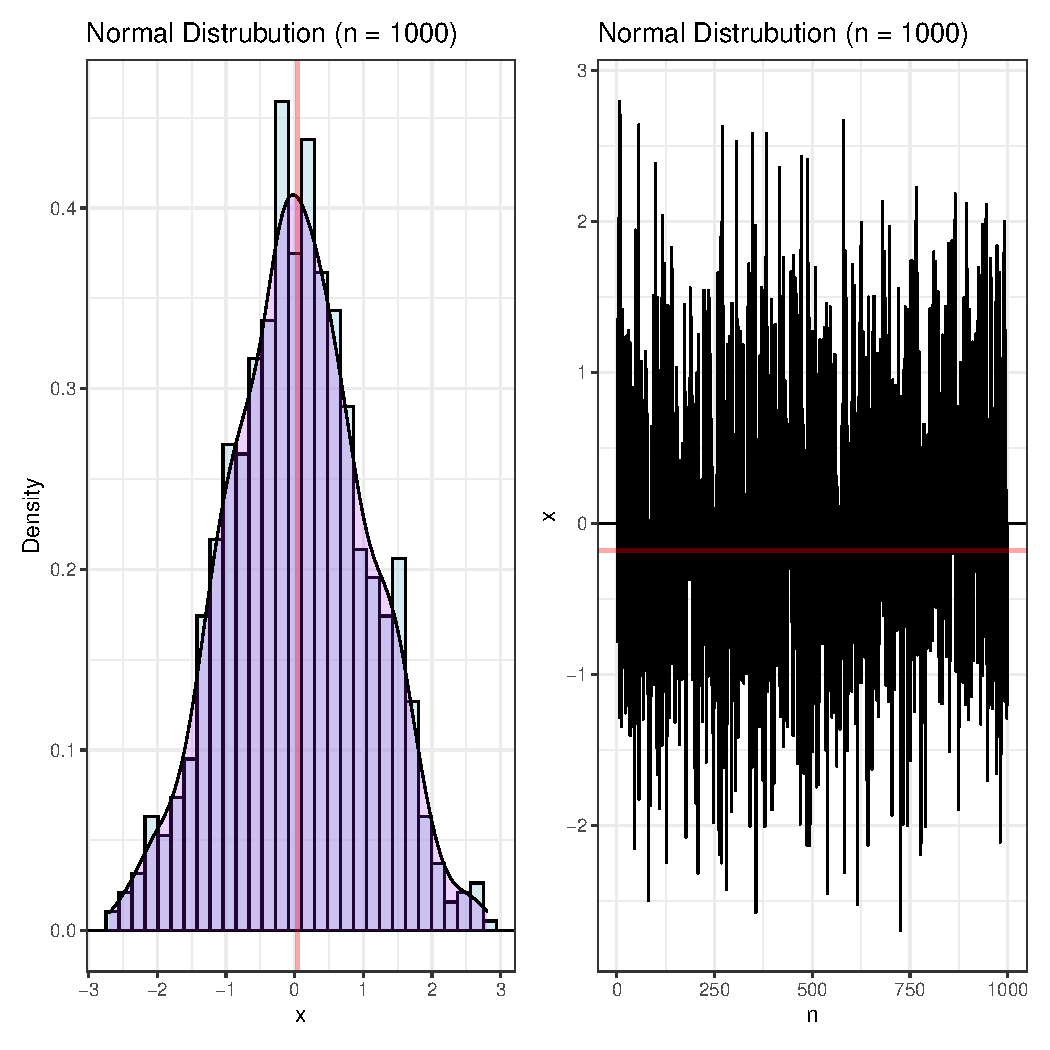
\includegraphics[width=\maxwidth]{figure/unnamed-chunk-33-2} 
\end{knitrout}
  %%%%%%%%%%%%%%%%%%%%%%%%%%%%%%%%%%%%%%%%%%%%%%%%%%%%%%%%%%%%%%%%%%%%%%%%%%%%%%%%%%%%%%%%%%%
  %%%%%%%%%  Part (g)
  %%%%%%%%%%%%%%%%%%%%%%%%%%%%%%%%%%%%%%%%%%%%%%%%%%%%%%%%%%%%%%%%%%%%%%%%%%%%%%%%%%%%%%%%%%%
  \item Comment on the results of parts (c)-(f). 
  
  Parts (c)-(f) illustrate the weak law of large numbers. As the sample size n increases, we see that both our computed estimators (MOM and MLE) tend to overlap more with their corresponding probability distributions - there is very less overlap when n = 10; however, at n = 1000, both the histograms are essentially superimposed on top of one another. Thus, as the sample size increases, our estimators do a better job at estimating the population statistics of the Normal distribution. We also notice that as the sample size increases, the sample mean gets closer to 0.
  
\end{enumerate}
\newpage
%%%%%%%%%%%%%%%%%%%%%%%%%%%%%%%%%%%%%%%%%%%%%%%%%%%%%%%%%%%%%%%%%%%%%%%%%%%%%%%%%%%%%%%%%%%
%%%%%%%%%%%%%%%%%%%%%%%%%%%%%%%%%%%%%%%%%%%%%%%%%%%%%%%%%%%%%%%%%%%%%%%%%%%%%%%%%%%%%%%%%%%
%%%%%%%%%  Question 3
%%%%%%%%%%%%%%%%%%%%%%%%%%%%%%%%%%%%%%%%%%%%%%%%%%%%%%%%%%%%%%%%%%%%%%%%%%%%%%%%%%%%%%%%%%%
%%%%%%%%%%%%%%%%%%%%%%%%%%%%%%%%%%%%%%%%%%%%%%%%%%%%%%%%%%%%%%%%%%%%%%%%%%%%%%%%%%%%%%%%%%%
  \item\label{Q3} Select a discrete distribution (not the Poisson). It does not 
  have to be one that we cover in the notes! To explore the PMF of your distribution, 
  specify two sets of parameter(s) for your distribution.
  \begin{enumerate}
  %%%%%%%%%%%%%%%%%%%%%%%%%%%%%%%%%%%%%%%%%%%%%%%%%%%%%%%%%%%%%%%%%%%%%%%%%%%%%%%%%%%%%%%%%%%
  %%%%%%%%%  Part (a)
  %%%%%%%%%%%%%%%%%%%%%%%%%%%%%%%%%%%%%%%%%%%%%%%%%%%%%%%%%%%%%%%%%%%%%%%%%%%%%%%%%%%%%%%%%%%
  \item \textbf{History} Discuss what types of random variables are modeled with 
  your distribution. Be sure to include a discussion about the support and ensure
  to provide the mass function, and CDF. This requires some internet research -- 
  what's the history of the distribution, why was it created and named? What are
  some exciting applications of this distribution? Cite all of your sources.
  %%%%%%%%%%%%%%%%%%%%%%%%%%%%%%%%%%%%%%%%%%%%%%%%%%%%%%%%%%%%%%%%%%%%%%%%%%%%%%%%%%%%%%%%%%%
  %%%%%%%%%  Part (b)
  %%%%%%%%%%%%%%%%%%%%%%%%%%%%%%%%%%%%%%%%%%%%%%%%%%%%%%%%%%%%%%%%%%%%%%%%%%%%%%%%%%%%%%%%%%%
	\item Show that you have a valid PMF. You can show this approximately by 
	calculating the series in a repeat loop until probability mass evaluations are 
	infinitesimally small.
	%%%%%%%%%%%%%%%%%%%%%%%%%%%%%%%%%%%%%%%%%%%%%%%%%%%%%%%%%%%%%%%%%%%%%%%%%%%%%%%%%%%%%%%%%%%
  %%%%%%%%%  Part (c)
  %%%%%%%%%%%%%%%%%%%%%%%%%%%%%%%%%%%%%%%%%%%%%%%%%%%%%%%%%%%%%%%%%%%%%%%%%%%%%%%%%%%%%%%%%%%
	\item Find the median for your two sets of parameter(s). Conduct some research 
	to find the median based on our PMF to confirm that your numerical approach is
	correct. 
	%%%%%%%%%%%%%%%%%%%%%%%%%%%%%%%%%%%%%%%%%%%%%%%%%%%%%%%%%%%%%%%%%%%%%%%%%%%%%%%%%%%%%%%%%%%
  %%%%%%%%%  Part (d)
  %%%%%%%%%%%%%%%%%%%%%%%%%%%%%%%%%%%%%%%%%%%%%%%%%%%%%%%%%%%%%%%%%%%%%%%%%%%%%%%%%%%%%%%%%%%
	\item \label{q3PMF} Graph the PMF for several values of the parameter(s) 
	including the two sets you specified. What does changing the parameter(s) do 
	to the shape of the PMF?
	%%%%%%%%%%%%%%%%%%%%%%%%%%%%%%%%%%%%%%%%%%%%%%%%%%%%%%%%%%%%%%%%%%%%%%%%%%%%%%%%%%%%%%%%%%%
  %%%%%%%%%  Part (e)
  %%%%%%%%%%%%%%%%%%%%%%%%%%%%%%%%%%%%%%%%%%%%%%%%%%%%%%%%%%%%%%%%%%%%%%%%%%%%%%%%%%%%%%%%%%%
	 \item Graph the CDF for the same values of the parameter(s) as you did in 
	 Question \ref{q3PMF}. What does changing the parameter(s) do to the shape of 
	 the CDF? Comment on the aspects of the CDFs that show that the CDF is valid.
	%%%%%%%%%%%%%%%%%%%%%%%%%%%%%%%%%%%%%%%%%%%%%%%%%%%%%%%%%%%%%%%%%%%%%%%%%%%%%%%%%%%%%%%%%%%
  %%%%%%%%%  Part (f)
  %%%%%%%%%%%%%%%%%%%%%%%%%%%%%%%%%%%%%%%%%%%%%%%%%%%%%%%%%%%%%%%%%%%%%%%%%%%%%%%%%%%%%%%%%%%
  \item Generate a random sample of size $n=10, 25, 100$, and $1000$ for your 
  two sets of parameter(s). In a $4 \times 2$ grid, plot a histogram (with bin 
  size 1) of each set of data and superimpose the true mass function at the 
  specified parameter values. Interpret the results.
	\end{enumerate}
%%%%%%%%%%%%%%%%%%%%%%%%%%%%%%%%%%%%%%%%%%%%%%%%%%%%%%%%%%%%%%%%%%%%%%%%%%%%%%%%%%%%%%%%%%%
%%%%%%%%%%%%%%%%%%%%%%%%%%%%%%%%%%%%%%%%%%%%%%%%%%%%%%%%%%%%%%%%%%%%%%%%%%%%%%%%%%%%%%%%%%%
%%%%%%%%%  Question 2
%%%%%%%%%%%%%%%%%%%%%%%%%%%%%%%%%%%%%%%%%%%%%%%%%%%%%%%%%%%%%%%%%%%%%%%%%%%%%%%%%%%%%%%%%%%
%%%%%%%%%%%%%%%%%%%%%%%%%%%%%%%%%%%%%%%%%%%%%%%%%%%%%%%%%%%%%%%%%%%%%%%%%%%%%%%%%%%%%%%%%%%
\item Continue with the discrete distribution you selected for Question \ref{Q3}.
\begin{enumerate}
  %%%%%%%%%%%%%%%%%%%%%%%%%%%%%%%%%%%%%%%%%%%%%%%%%%%%%%%%%%%%%%%%%%%%%%%%%%%%%%%%%%%%%%%%%%%
  %%%%%%%%%  Part (a)
  %%%%%%%%%%%%%%%%%%%%%%%%%%%%%%%%%%%%%%%%%%%%%%%%%%%%%%%%%%%%%%%%%%%%%%%%%%%%%%%%%%%%%%%%%%%
  \item Provide the mean, standard deviation, skewness, and kurtosis of the PMF. 
  Ensure to interpret each.
  %%%%%%%%%%%%%%%%%%%%%%%%%%%%%%%%%%%%%%%%%%%%%%%%%%%%%%%%%%%%%%%%%%%%%%%%%%%%%%%%%%%%%%%%%%%
  %%%%%%%%%  Part (b)
  %%%%%%%%%%%%%%%%%%%%%%%%%%%%%%%%%%%%%%%%%%%%%%%%%%%%%%%%%%%%%%%%%%%%%%%%%%%%%%%%%%%%%%%%%%%
  \item Generate a random sample of size $n=10, 25, 100$, and $1000$ for your 
  two sets of parameter(s). Calculate the sample mean, standard deviation, 
  skewness, and kurtosis. Interpret the results.
  %%%%%%%%%%%%%%%%%%%%%%%%%%%%%%%%%%%%%%%%%%%%%%%%%%%%%%%%%%%%%%%%%%%%%%%%%%%%%%%%%%%%%%%%%%%
  %%%%%%%%%  Part (c)
  %%%%%%%%%%%%%%%%%%%%%%%%%%%%%%%%%%%%%%%%%%%%%%%%%%%%%%%%%%%%%%%%%%%%%%%%%%%%%%%%%%%%%%%%%%%
  \item Generate a random sample of size $n=10$ for your two sets of parameter(s).
  Calculate the method of moments estimator(s) and maximum likelihood estimator(s).
  In a $1 \times 2$ grid, plot a histogram (with bin size 1) of each set of data 
  with (1) the method of moments estimated distribution, (2) the maximum likelihood 
  estimated distribution, and superimpose the true distribution in both.
  %%%%%%%%%%%%%%%%%%%%%%%%%%%%%%%%%%%%%%%%%%%%%%%%%%%%%%%%%%%%%%%%%%%%%%%%%%%%%%%%%%%%%%%%%%%
  %%%%%%%%%  Part (d)
  %%%%%%%%%%%%%%%%%%%%%%%%%%%%%%%%%%%%%%%%%%%%%%%%%%%%%%%%%%%%%%%%%%%%%%%%%%%%%%%%%%%%%%%%%%%
  \item Generate a random sample of size $n=25$ for your two sets of parameter(s). 
  Calculate the method of moments estimator(s) and maximum likelihood estimator(s).
  In a $1 \times 2$ grid, plot a histogram (with bin size 1) of each set of data 
  with (1) the method of moments estimated distribution, (2) the maximum likelihood 
  estimated distribution, and superimpose the true distribution in both.
  %%%%%%%%%%%%%%%%%%%%%%%%%%%%%%%%%%%%%%%%%%%%%%%%%%%%%%%%%%%%%%%%%%%%%%%%%%%%%%%%%%%%%%%%%%%
  %%%%%%%%%  Part (e)
  %%%%%%%%%%%%%%%%%%%%%%%%%%%%%%%%%%%%%%%%%%%%%%%%%%%%%%%%%%%%%%%%%%%%%%%%%%%%%%%%%%%%%%%%%%%
  \item Generate a random sample of size $n=100$ for your two sets of parameter(s).
  Calculate the method of moments estimator(s) and maximum likelihood estimator(s). 
  In a $1 \times 2$ grid, plot a histogram (with bin size 1) of each set of data 
  with (1) the method of moments estimated distribution, (2) the maximum likelihood
  estimated distribution, and superimpose the true distribution in both.
  %%%%%%%%%%%%%%%%%%%%%%%%%%%%%%%%%%%%%%%%%%%%%%%%%%%%%%%%%%%%%%%%%%%%%%%%%%%%%%%%%%%%%%%%%%%
  %%%%%%%%%  Part (f)
  %%%%%%%%%%%%%%%%%%%%%%%%%%%%%%%%%%%%%%%%%%%%%%%%%%%%%%%%%%%%%%%%%%%%%%%%%%%%%%%%%%%%%%%%%%%
  \item Generate a random sample of size $n=100$ for your two sets of parameter(s).
  Calculate the method of moments estimator(s) and maximum likelihood estimator(s).
  In a $1 \times 2$ grid, plot a histogram (with bin size 1) of each set of data 
  with (1) the method of moments estimated distribution, (2) the maximum likelihood
  estimated distribution, and superimpose the true distribution in both.
  %%%%%%%%%%%%%%%%%%%%%%%%%%%%%%%%%%%%%%%%%%%%%%%%%%%%%%%%%%%%%%%%%%%%%%%%%%%%%%%%%%%%%%%%%%%
  %%%%%%%%%  Part (g)
  %%%%%%%%%%%%%%%%%%%%%%%%%%%%%%%%%%%%%%%%%%%%%%%%%%%%%%%%%%%%%%%%%%%%%%%%%%%%%%%%%%%%%%%%%%%
  \item Comment on the results of parts (c)-(f). 
\end{enumerate}
\end{enumerate}%End overall enumerate
\newpage
\bibliography{bib}
\end{document}
